
\documentclass[aspectratio=169,10pt,english]{beamer} 
\usepackage[utf8]{inputenc} 

\usepackage{beamer}

\urlstyle{same}

\usepackage[export]{adjustbox}

\usepackage{booktabs}
\usepackage{graphicx}
\usepackage{csquotes}
\usepackage{pdfpages}
\usepackage{gensymb}
\usepackage{hyperref}
\usepackage{tabto}
\usepackage{tikz}
\usetikzlibrary{calc,positioning,spy}

\setbeamertemplate{frametitle continuation}{\insertcontinuationcount}

\usepackage{siunitx}

\newcommand{\colorbitbox}[3]{%
  \sbox0{\bitbox{#2}{#3}}%
  \makebox[0pt][l]{\textcolor{#1}{\rule[-\dp0]{\wd0}{\ht0}}}%
  \bitbox{#2}{#3}%
}

\usepackage[endianness=big]{bytefield}
\bytefieldsetup{boxformatting={\centering\footnotesize}} 
\usepackage{amsmath}

\newlength{\maxheight}
\setlength{\maxheight}{\heightof{W}}
\newcommand{\baselinealign}[1]{%
    \centering
    \raisebox{0pt}[\maxheight][0pt]{#1}%
}

\usepackage{xcolor}

\usetikzlibrary{calc,positioning,spy,shapes.misc}

\tikzset{
  rectangle with rounded corners north west/.initial=4pt,
  rectangle with rounded corners south west/.initial=4pt,
  rectangle with rounded corners north east/.initial=4pt,
  rectangle with rounded corners south east/.initial=4pt,
}
\makeatletter
\pgfdeclareshape{rectangle with rounded corners}{
  \inheritanchorborder[from=rectangle]
  \savedmacro{\neoffset}{
    \pgfkeysgetvalue{/tikz/rectangle with rounded corners north east}{\pgf@rectc}
    \let\neoffset\pgf@rectc
  }
  \savedmacro{\nwoffset}{
    \pgfkeysgetvalue{/tikz/rectangle with rounded corners north west}{\pgf@rectc}
    \let\nwoffset\pgf@rectc
  }
  \savedmacro{\seoffset}{
    \pgfkeysgetvalue{/tikz/rectangle with rounded corners south east}{\pgf@rectc}
    \let\seoffset\pgf@rectc
  }
  \savedmacro{\swoffset}{
    \pgfkeysgetvalue{/tikz/rectangle with rounded corners south west}{\pgf@rectc}
    \let\swoffset\pgf@rectc
  }
  \savedanchor{\north}{
    \pgf@y=.5\ht\pgfnodeparttextbox
    \pgf@x=0pt
    \setlength{\pgf@ya}{\pgfshapeminheight}
    \ifdim\pgf@y<.5\pgf@ya
      \pgf@y=.5\pgf@ya
    \fi
  }
  \savedanchor{\south}{
    \pgf@y=-.5\ht\pgfnodeparttextbox
    \pgf@x=0pt
    \setlength{\pgf@ya}{\pgfshapeminheight}
    \ifdim\pgf@y>-.5\pgf@ya
      \pgf@y=-.5\pgf@ya
    \fi
  }
  \savedanchor{\east}{
    \pgf@y=0pt
    \pgf@x=.5\wd\pgfnodeparttextbox
    \addtolength{\pgf@x}{2ex}
    \setlength{\pgf@xa}{\pgfshapeminwidth}
    \ifdim\pgf@x<.5\pgf@xa
      \pgf@x=.5\pgf@xa
    \fi
  }
  \savedanchor{\west}{
    \pgf@y=0pt
    \pgf@x=-.5\wd\pgfnodeparttextbox
    \addtolength{\pgf@x}{-2ex}
    \setlength{\pgf@xa}{\pgfshapeminwidth}
    \ifdim\pgf@x>-.5\pgf@xa
      \pgf@x=-.5\pgf@xa
    \fi
  }
  \savedanchor{\northeast}{
    \pgf@y=.5\ht\pgfnodeparttextbox %
    \pgf@x=.5\wd\pgfnodeparttextbox %
    \addtolength{\pgf@x}{2ex}
    \setlength{\pgf@xa}{\pgfshapeminwidth}
    \ifdim\pgf@x<.5\pgf@xa
      \pgf@x=.5\pgf@xa
    \fi
    \setlength{\pgf@ya}{\pgfshapeminheight}
    \ifdim\pgf@y<.5\pgf@ya
      \pgf@y=.5\pgf@ya
    \fi
  }
  \savedanchor{\southwest}{
    \pgf@y=-.5\ht\pgfnodeparttextbox
    \pgf@x=-.5\wd\pgfnodeparttextbox
    \addtolength{\pgf@x}{-2ex}
    \setlength{\pgf@xa}{\pgfshapeminwidth}
    \ifdim\pgf@x>-.5\pgf@xa
      \pgf@x=-.5\pgf@xa
    \fi
    \setlength{\pgf@ya}{\pgfshapeminheight}
    \ifdim\pgf@y>-.5\pgf@ya
      \pgf@y=-.5\pgf@ya
    \fi
  }
  \anchor{text}{%
    \northeast%
    \pgf@x=-.5\wd\pgfnodeparttextbox%
    \pgfmathsetlength{\pgf@y}{-.5ex}
  }
  \anchor{north east}{
    \northeast
    \pgfmathsetmacro{\nw}{(1-sin(45))*\neoffset}
    \addtolength{\pgf@x}{-\nw pt}
    \addtolength{\pgf@y}{-\nw pt}
  }
  \anchor{center}{
    \pgf@x=0pt
    \pgf@y=0pt
  }
  \anchor{south west}{
    \southwest
    \pgfmathsetmacro{\nw}{(1-sin(45))*\swoffset}
    \addtolength{\pgf@x}{\nw pt}
    \addtolength{\pgf@y}{\nw pt}
  }
  \anchor{north west}{
    \northeast
    \pgfmathsetmacro{\temp@x}{\pgf@x}
    \southwest
    \pgfmathsetmacro{\temp@xtwo}{\pgf@x}
    \northeast
    \pgfmathsetmacro{\xdiff}{\temp@x-\temp@xtwo}
    \def\pgf@xa{\pgf@x-\xdiff}
            \pgfmathsetmacro{\nw}{(1-sin(45))*\nwoffset}
    \def\pgf@xaa{\pgf@xa+\nw}
    \def\pgf@yaa{\pgf@y-\nw}
    \pgfpoint{\pgf@xaa}{\pgf@yaa}
  }
  \anchor{south east}{
    \southwest
    \pgfmathsetmacro{\temp@x}{\pgf@x}
    \northeast
    \pgfmathsetmacro{\temp@xtwo}{\pgf@x}
    \southwest
    \pgfmathsetmacro{\xdiff}{\temp@x-\temp@xtwo}
    \def\pgf@xa{\pgf@x-\xdiff}
    \pgfmathsetmacro{\nw}{(1-sin(45))*\seoffset}
    \def\pgf@xaa{\pgf@xa-\nw}
    \def\pgf@yaa{\pgf@y+\nw}
    \pgfpoint{\pgf@xaa}{\pgf@yaa}
  }
  \anchor{south}{\south}
  \anchor{north}{\north}
  \anchor{east}{\east}
  \anchor{west}{\west}
  \backgroundpath{%
    \southwest \pgf@xa=\pgf@x \pgf@ya=\pgf@y
    \northeast \pgf@xb=\pgf@x \pgf@yb=\pgf@y
    \pgfkeysgetvalue{/tikz/rectangle with rounded corners north west}{\pgf@rectc}
    \pgfsetcornersarced{\pgfpoint{\pgf@rectc}{\pgf@rectc}}
    \pgfpathmoveto{\pgfpoint{\pgf@xa}{\pgf@ya}}
    \pgfpathlineto{\pgfpoint{\pgf@xa}{\pgf@yb}}
    \pgfkeysgetvalue{/tikz/rectangle with rounded corners north east}{\pgf@rectc}
    \pgfsetcornersarced{\pgfpoint{\pgf@rectc}{\pgf@rectc}}
    \pgfpathlineto{\pgfpoint{\pgf@xb}{\pgf@yb}}
    \pgfkeysgetvalue{/tikz/rectangle with rounded corners south east}{\pgf@rectc}
    \pgfsetcornersarced{\pgfpoint{\pgf@rectc}{\pgf@rectc}}
    \pgfpathlineto{\pgfpoint{\pgf@xb}{\pgf@ya}}
    \pgfkeysgetvalue{/tikz/rectangle with rounded corners south west}{\pgf@rectc}
    \pgfsetcornersarced{\pgfpoint{\pgf@rectc}{\pgf@rectc}}
    \pgfpathclose
 }
}
\makeatother

\usepackage{egweblnk}

\usepackage{caption}

\title{RoomCanvas: A Visualization System for Spatiotemporal Temperature Data in Smart Homes}
\subtitle{EuroVis 2021 Short Paper}
\author{B. König et al.}

\newcommand{\websource}[1]{\footnote[frame]{\href{#1}{#1}}}

\newcommand\barefootnotetext[1]{%
  \begingroup
  \renewcommand\thefootnote{}\footnote{#1}%
  \addtocounter{footnote}{-1}%
  \endgroup
}

\setbeamertemplate{bibliography item}{\insertbiblabel}

\begin{document} 

{
\usebackgroundtemplate{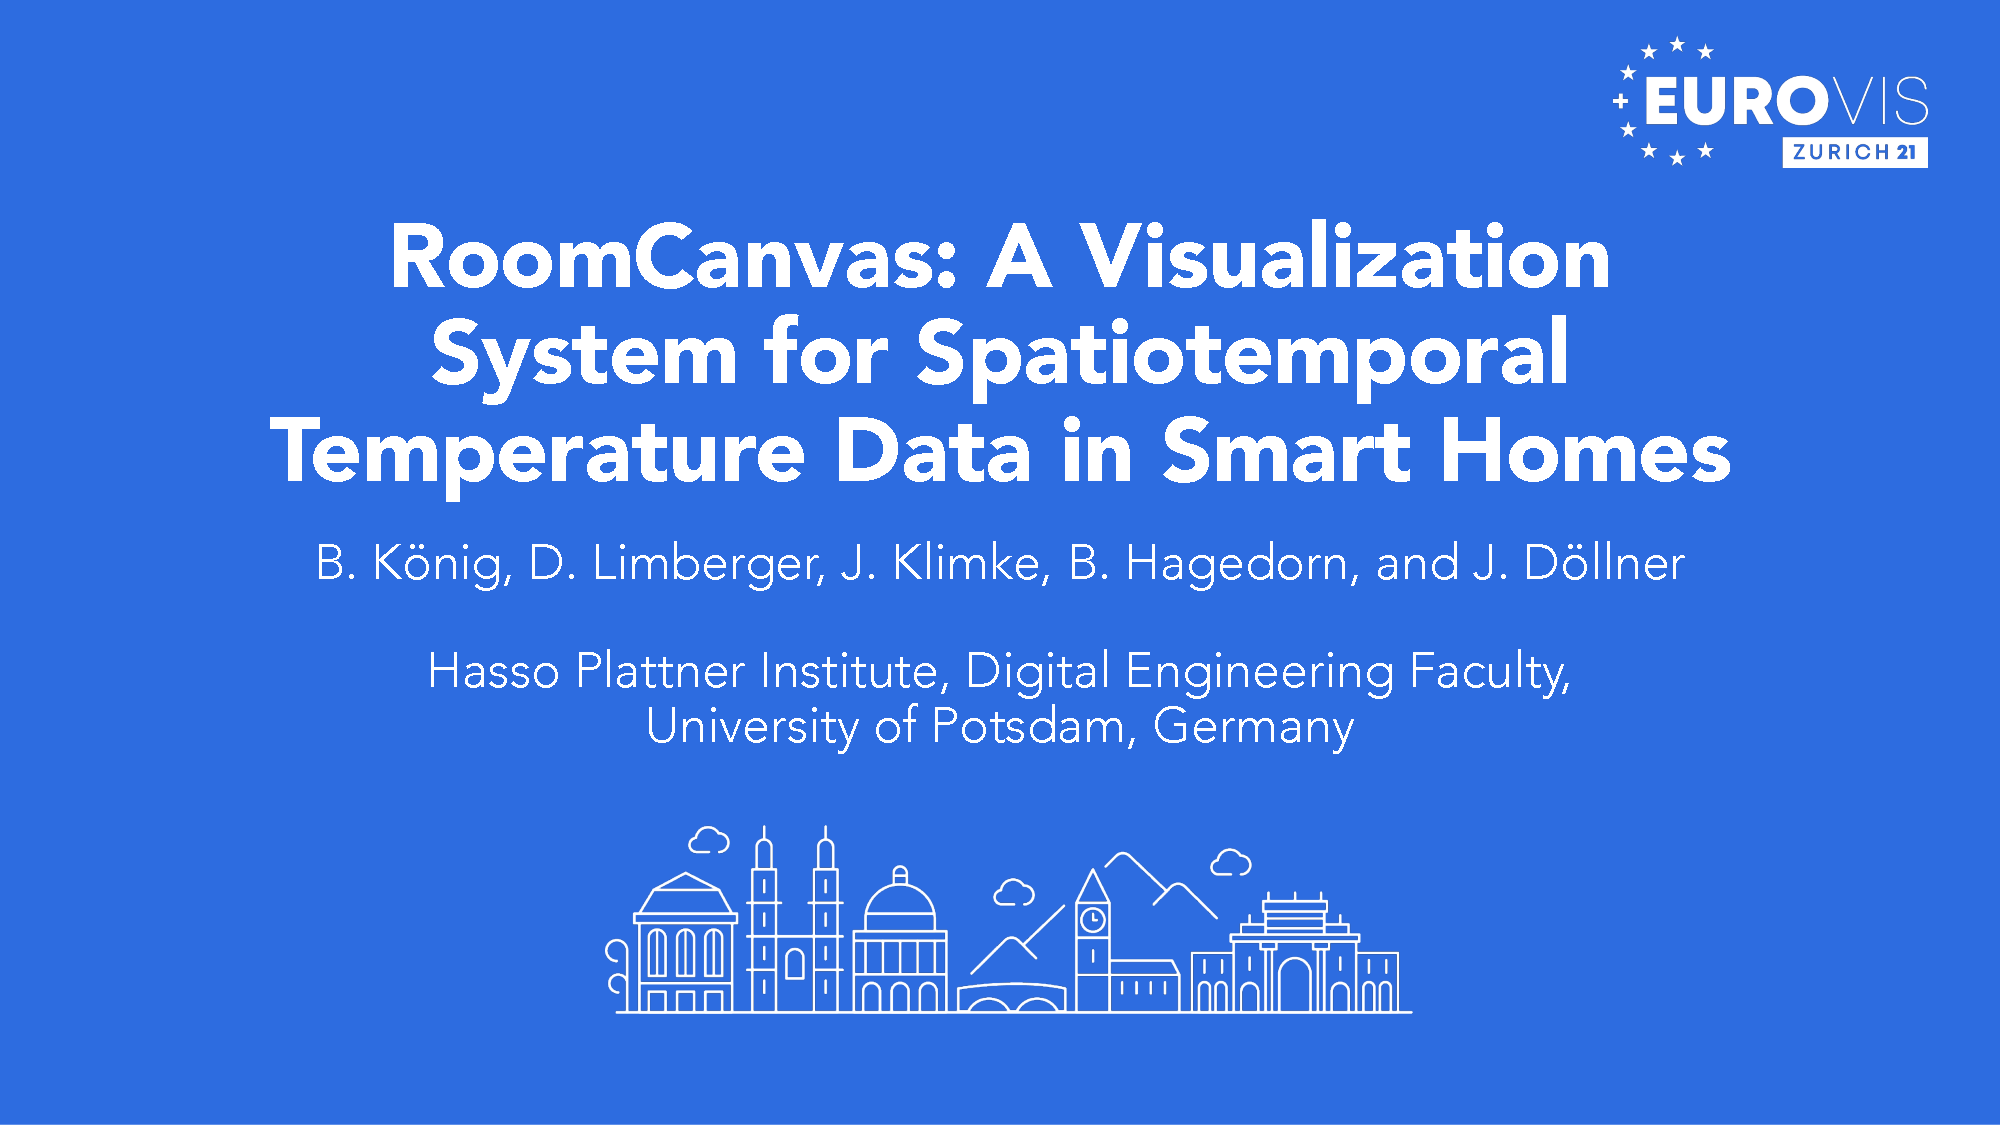
\includegraphics[width=\paperwidth]{figures/EuroVis21.pdf}}
\begin{frame}[plain]
\end{frame} 
}

\begin{frame}[t]{\textbf{Motivation}}

    \begin{columns}
        \begin{column}{0.618\textwidth}
        
            \begin{quote}
                \enquote{IoT systems often involve huge amounts of data from a wide variety of sources, including sensors. \textelp{} this data must be converted into decisions and actions.}~\cite{gartner-iot}
            \end{quote}
        
            \begin{itemize}
                \item Spatiotemporal sensor data is increasingly collected and made available in smart homes
                \item Data is sent to and analyzed by cloud services but often not available for consumer exploration
                \item Unified view of sensor data and the building environment allows for variety of use cases
            \end{itemize}
            \vspace{0.7em}
            \begin{itemize}
                \item Tools to explore, monitor, and understand spatiotemporal sensor data within their spatial and temporal context will become more important for experts and non-experts alike
            \end{itemize}
        \end{column}
        \begin{column}{0.332\textwidth}
            \vspace{0.7em}
            \begin{tikzpicture}
                \node[inner sep=0pt] (sensors-and-homekit) at (0,0)
                {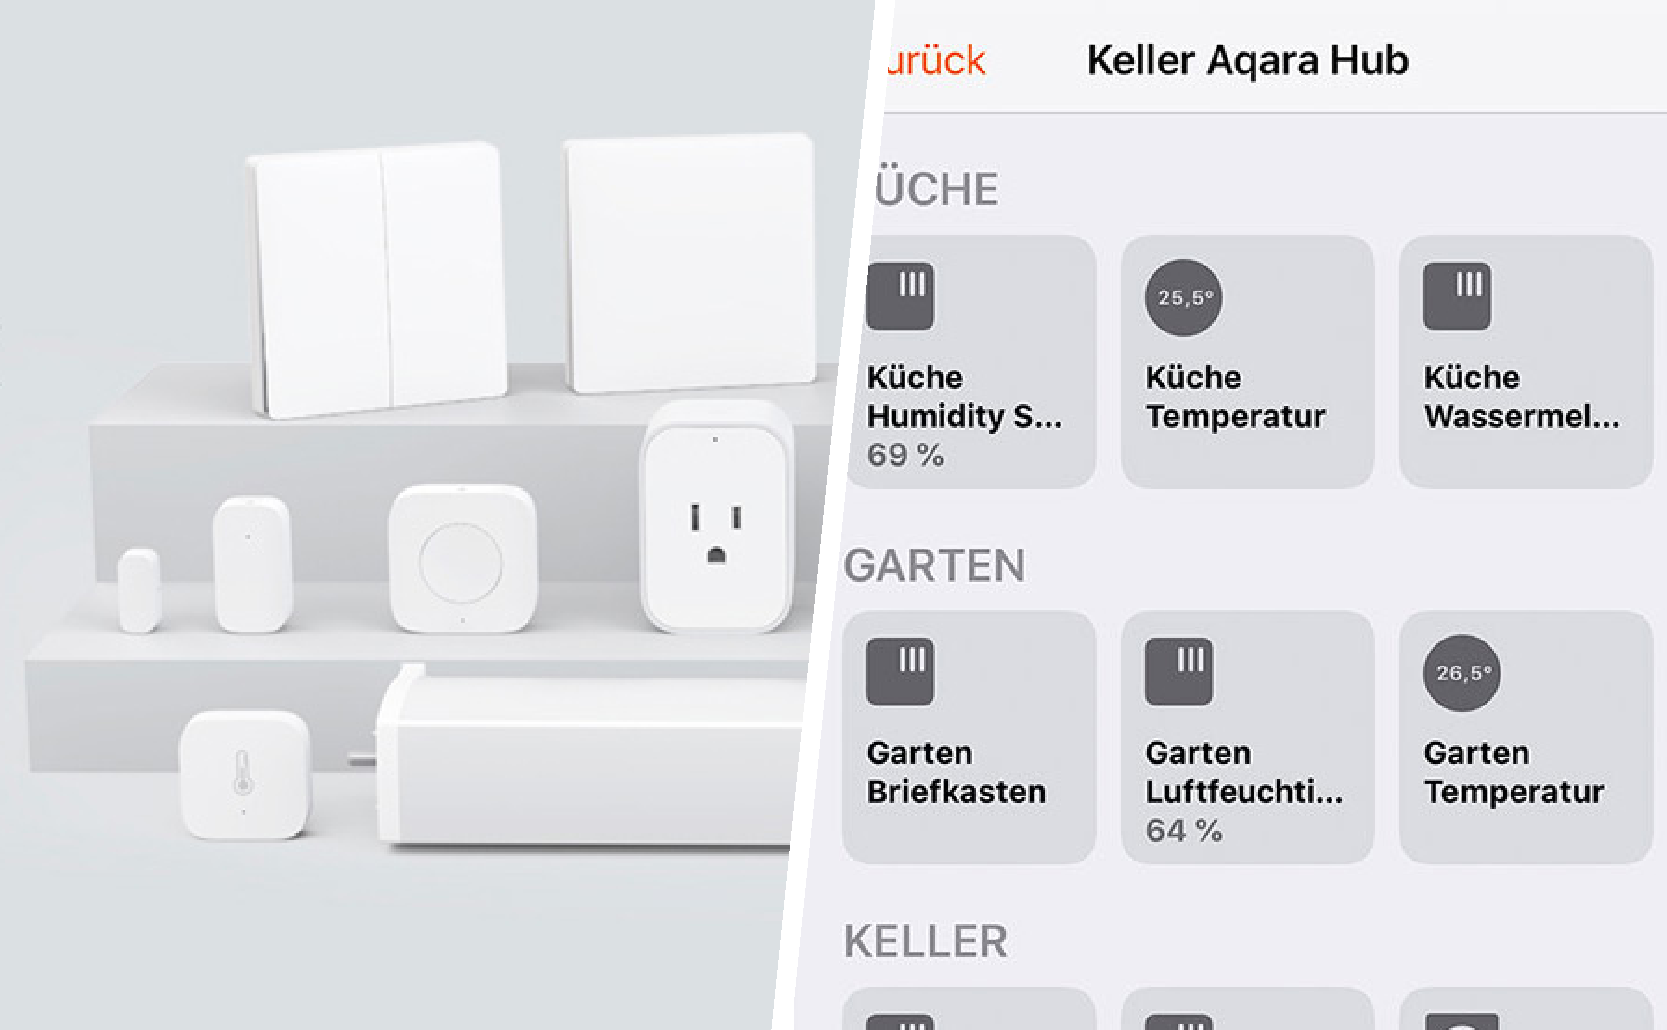
\includegraphics[width=\textwidth]{figures/motivation_1-sensors-homekit-v2}};
                \node[
                    minimum height=0.55cm,
                    minimum width=0.55cm,
                    anchor=south west,
                    fill=white,
                    shape=rectangle with rounded corners,
                    rectangle with rounded corners north west=0pt,
                    rectangle with rounded corners south west=0pt,
                    rectangle with rounded corners north east=2mm,
                    rectangle with rounded corners south east=0pt,
                    text width=0.53cm,
                ] at (sensors-and-homekit.south west) (sensors) {};
                \node[anchor=south west,inner sep=1pt] at (sensors.south west) 
                {\cite{aqara-sensors}};
                \node[
                    minimum height=0.55cm,
                    minimum width=0.55cm,
                    anchor=south east,
                    fill=white,
                    shape=rectangle with rounded corners,
                    rectangle with rounded corners north west=2mm,
                    rectangle with rounded corners south west=0pt,
                    rectangle with rounded corners north east=0pt,
                    rectangle with rounded corners south east=0pt,
                    text width=0.54cm,
                ] at (sensors-and-homekit.south east) (homekit) {};
                \node[anchor=south east,inner sep=1pt] at (homekit.south east) 
                {\cite{homekit-screenshot}};
            \end{tikzpicture}\\
            \begin{figure}
                \centering
                \begin{tikzpicture}
                    \node[inner sep=0pt] (related-work) at (0,0)
                    {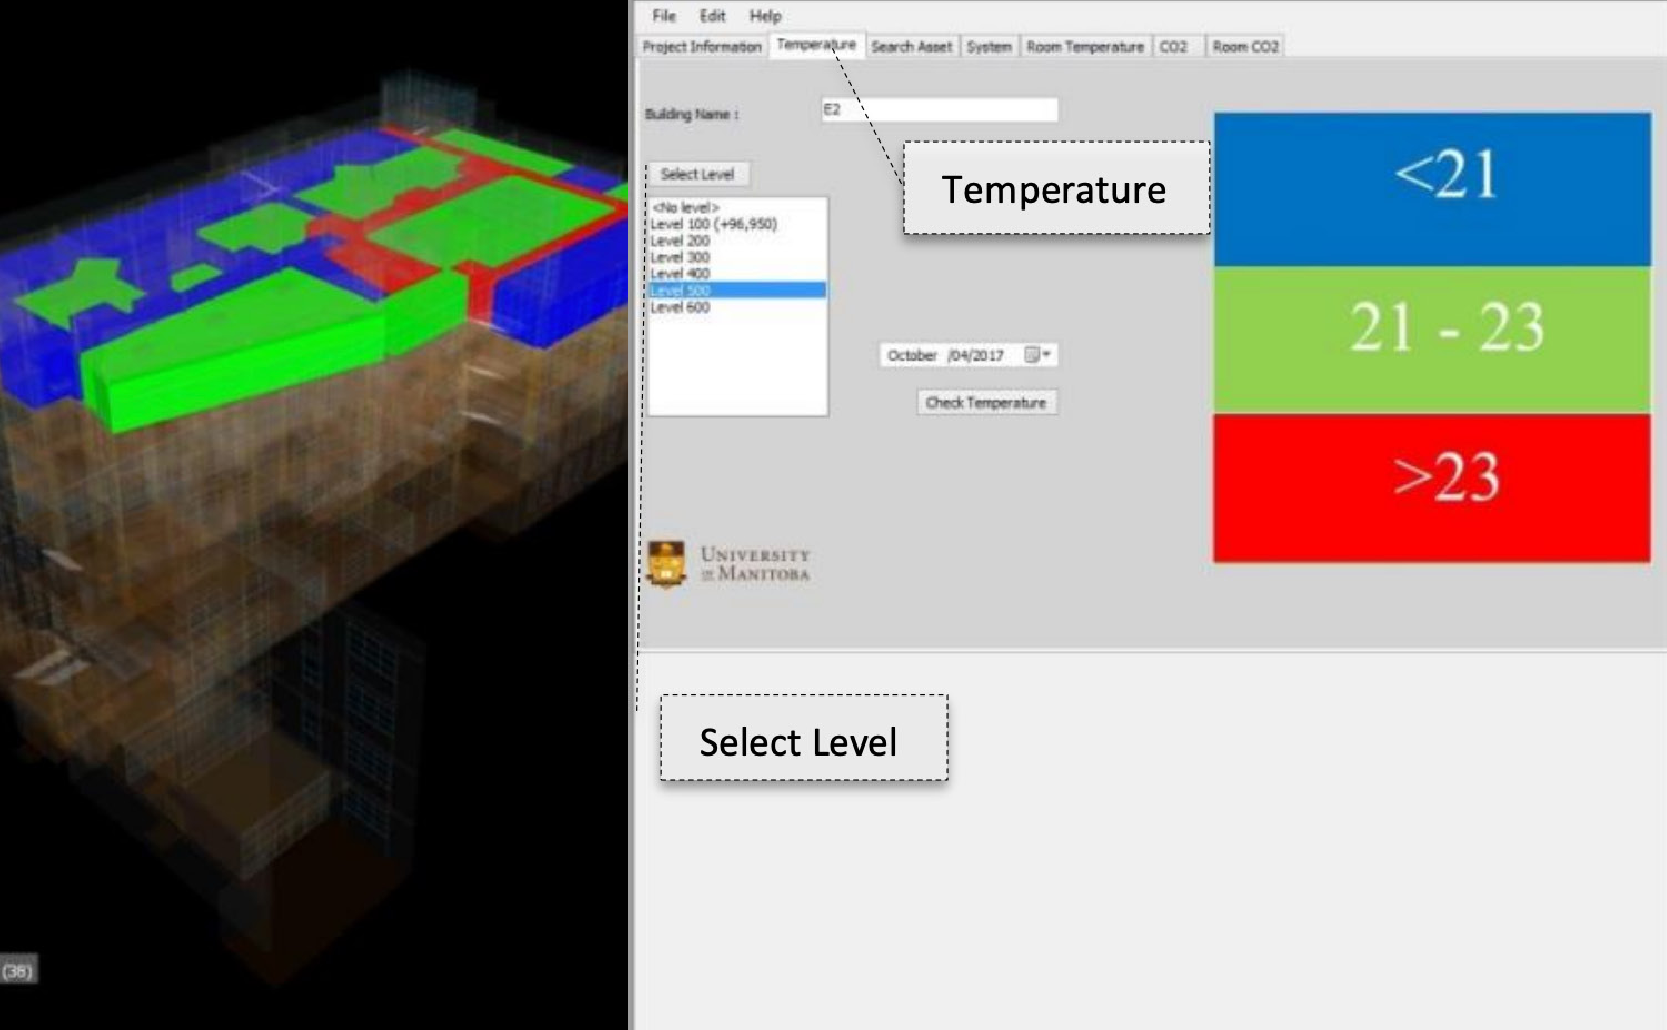
\includegraphics[trim=0 195 0 0, clip,width=\textwidth]{figures/motivation_2-related-work}};
                    \node[
                        minimum height=0.55cm,
                        minimum width=0.55cm,
                        anchor=south west,
                        fill=white,
                        shape=rectangle with rounded corners,
                        rectangle with rounded corners north west=0pt,
                        rectangle with rounded corners south west=0pt,
                        rectangle with rounded corners north east=2mm,
                        rectangle with rounded corners south east=0pt,
                        text width=0.62cm,
                    ] at (related-work.south west) (bg) {};
                    \node[anchor=south west,inner sep=1pt] at (bg.south west) 
                    {\cite{kazado_integrating_2019}};
                \end{tikzpicture}\\
                \caption*{Existing systems: Often tightly coupled to expert CAD software}
            \end{figure}
        \end{column}
    \end{columns}

\end{frame}

\begin{frame}[t]{Demo\enspace{}|\enspace{}\textbf{Interactive, Web-based Visualization System}}

    \begin{columns}[T]
        \begin{column}{0.60\textwidth}
            \begin{figure}
                \centering
                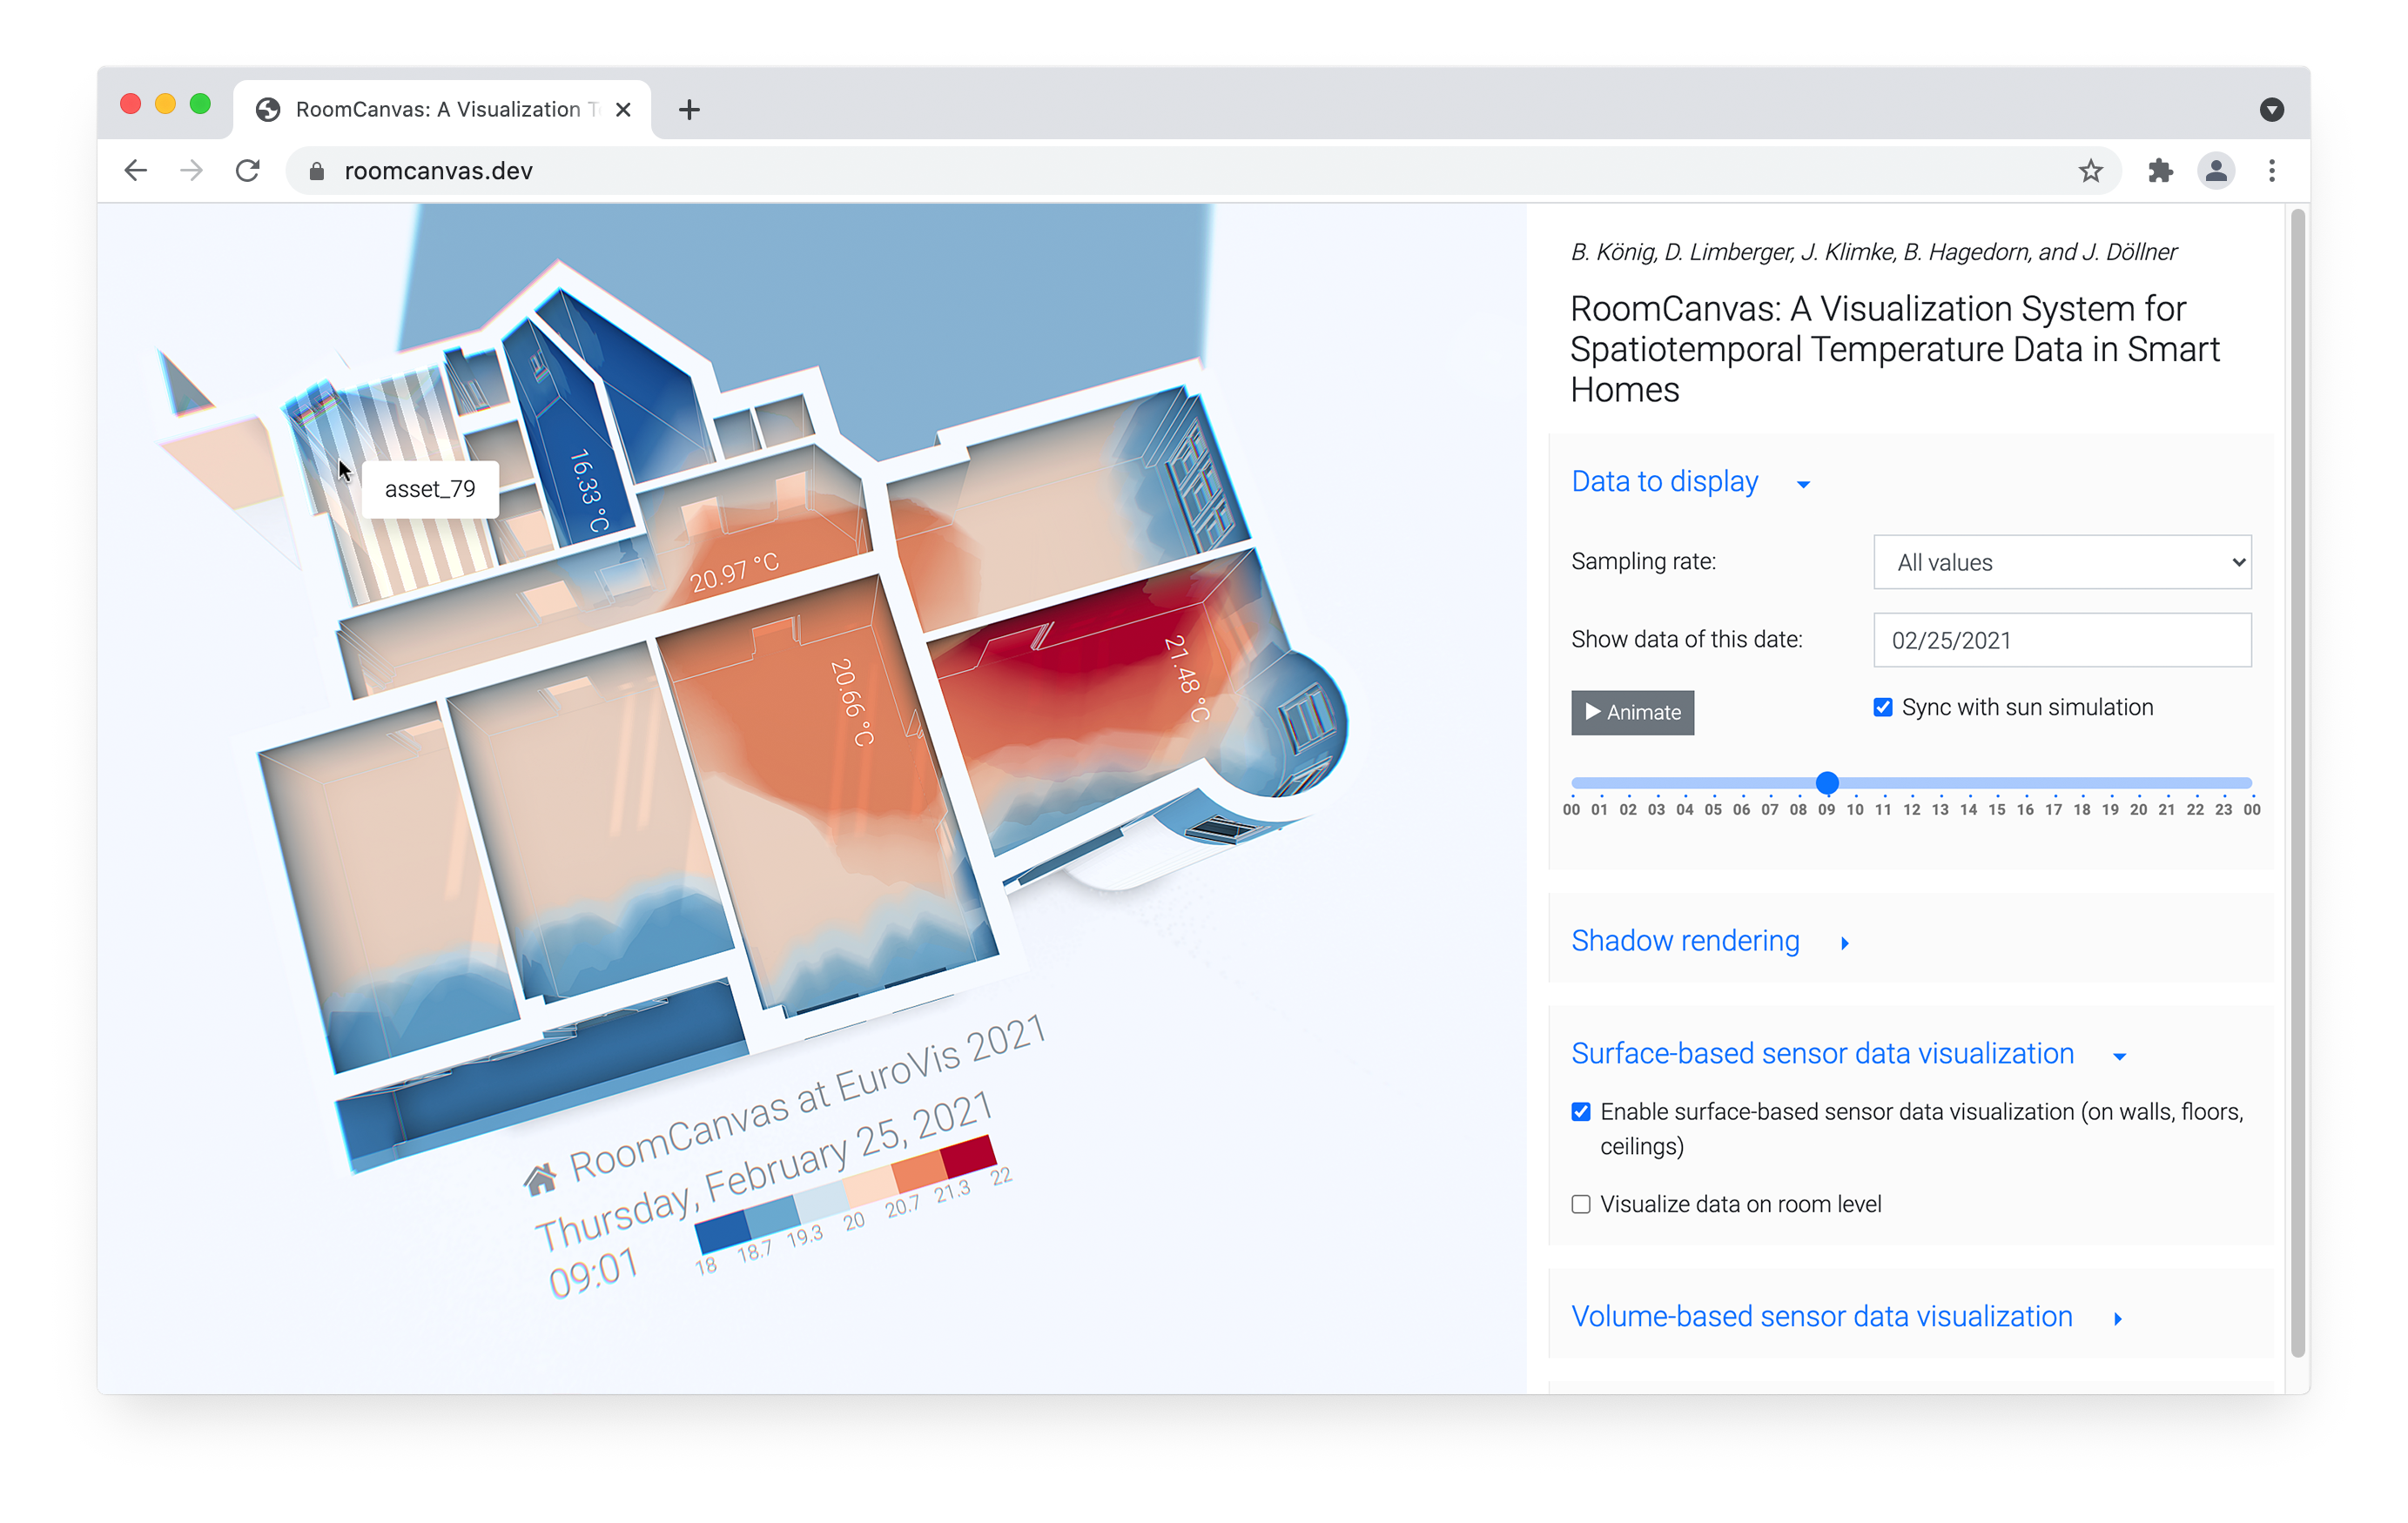
\includegraphics[width=1.0\textwidth]{figures/demo_preview.png}
                \vspace*{-2.5em}
                \caption*{You can try it out for yourself at \url{https://roomcanvas.dev}.}
            \end{figure}
        \end{column}
        
        \begin{column}{0.32\textwidth}
            \vspace{2.5em}
            Source code for both the web-based visualization and the server-side preprocessing is open sourced and available at\\
            \vspace{0.5em}
            
\includegraphics[valign=m,width=1.2em]{figures/GitHub-Mark__small_16-120px.pdf}~~ \href{https://github.com/varg-dev/roomcanvas}{varg-dev\,/\,\textbf{roomcanvas}}
        \end{column}
    \end{columns}

\end{frame}

\begin{frame}[t]{System Details\enspace{}|\enspace{}\textbf{Overview}}

    \vspace{1.5em}
    \begin{figure}
        \centering
        \only<1>{%
            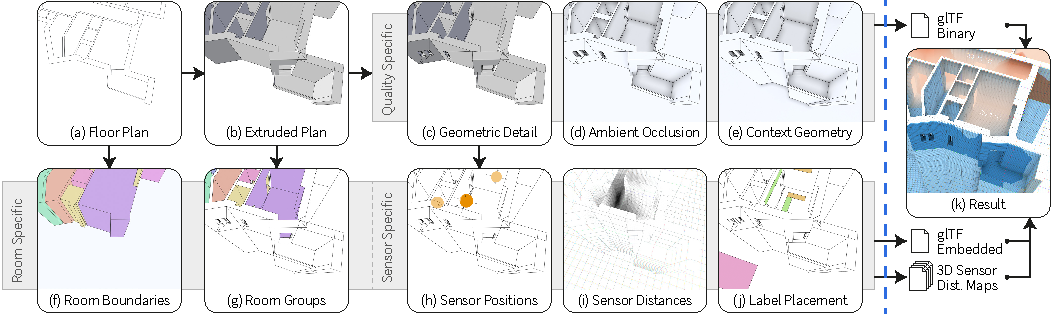
\includegraphics[width=1.0\textwidth]{figures/components-overview_source-sans-pro-600dpi.pdf}
            \caption*{\hspace{4cm}Server-side preprocessing\hspace{5cm}Web client}}%
        \only<2>{%
            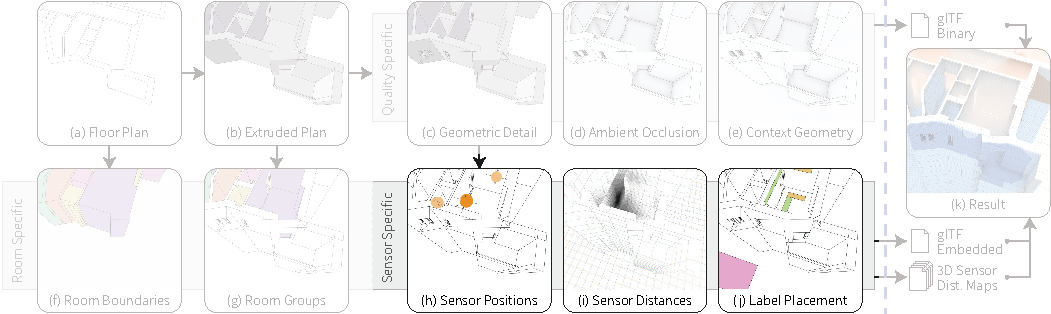
\includegraphics[width=1.0\textwidth]{figures/components-overview_source-sans-pro-600dpi-focus.pdf}
            \caption*{\hspace{4cm}Server-side preprocessing\hspace{5cm}Web client}}%
    \end{figure}

\end{frame}

\begin{frame}[t]{System Details\enspace{}|\enspace{}\textbf{Per-Sensor Distance Map Computation}}

    \begin{columns}[T]
        \begin{column}{0.4\textwidth}

            Precomputation of 3D distance maps for each sensor to allow for boundary-aware sensor data interpolation:
            \medskip

            \only<2->{%
            \begin{enumerate}\small
                \only<2->{%
                \item Create a voxelized cuboid around the building model%
                }
                \only<3->{%
                \item Flag any voxels intersecting with boundary elements, i.e., polygons of walls, floors, and ceilings%
                }
                \only<4->{%
                \item Use a modified flood fill algorithm to create a 16-bit distance map for each sensor, taking cells flagged as boundary into account%
                }
            \end{enumerate}
            }

        \end{column}
        \begin{column}{0.54\textwidth}

            \only<1>{
                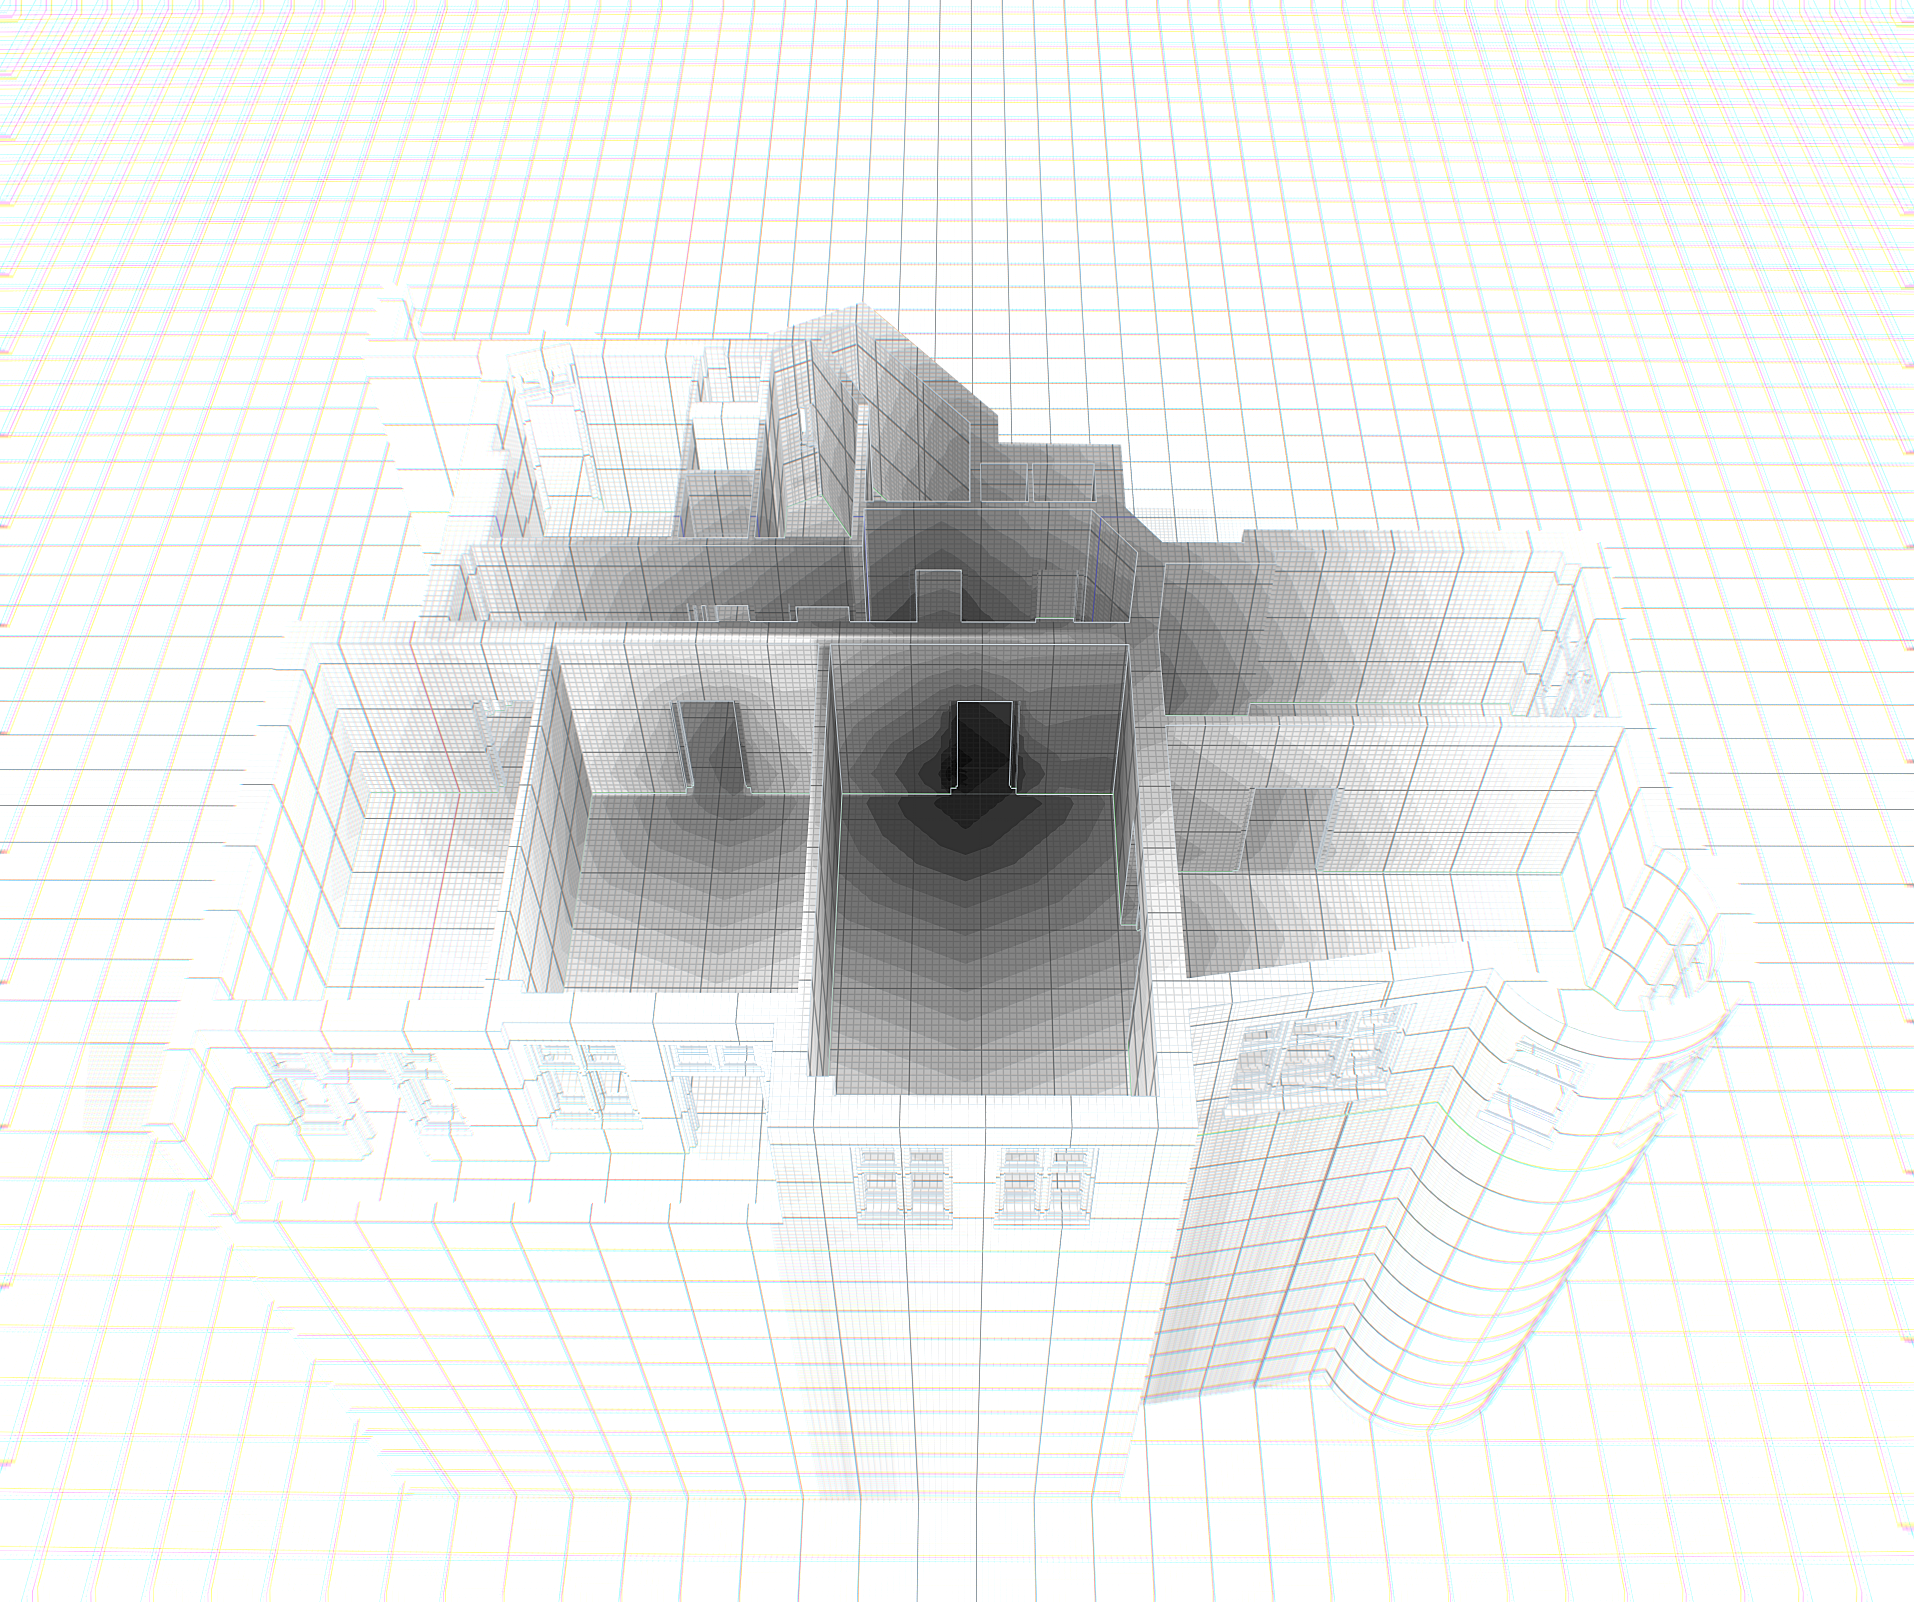
\includegraphics[trim=20 20 20 100, clip,width=\textwidth]{figures/debug_sensor_distances_roomcanvas.png}
            }
            \only<2>{
                \vspace{0.5em}
                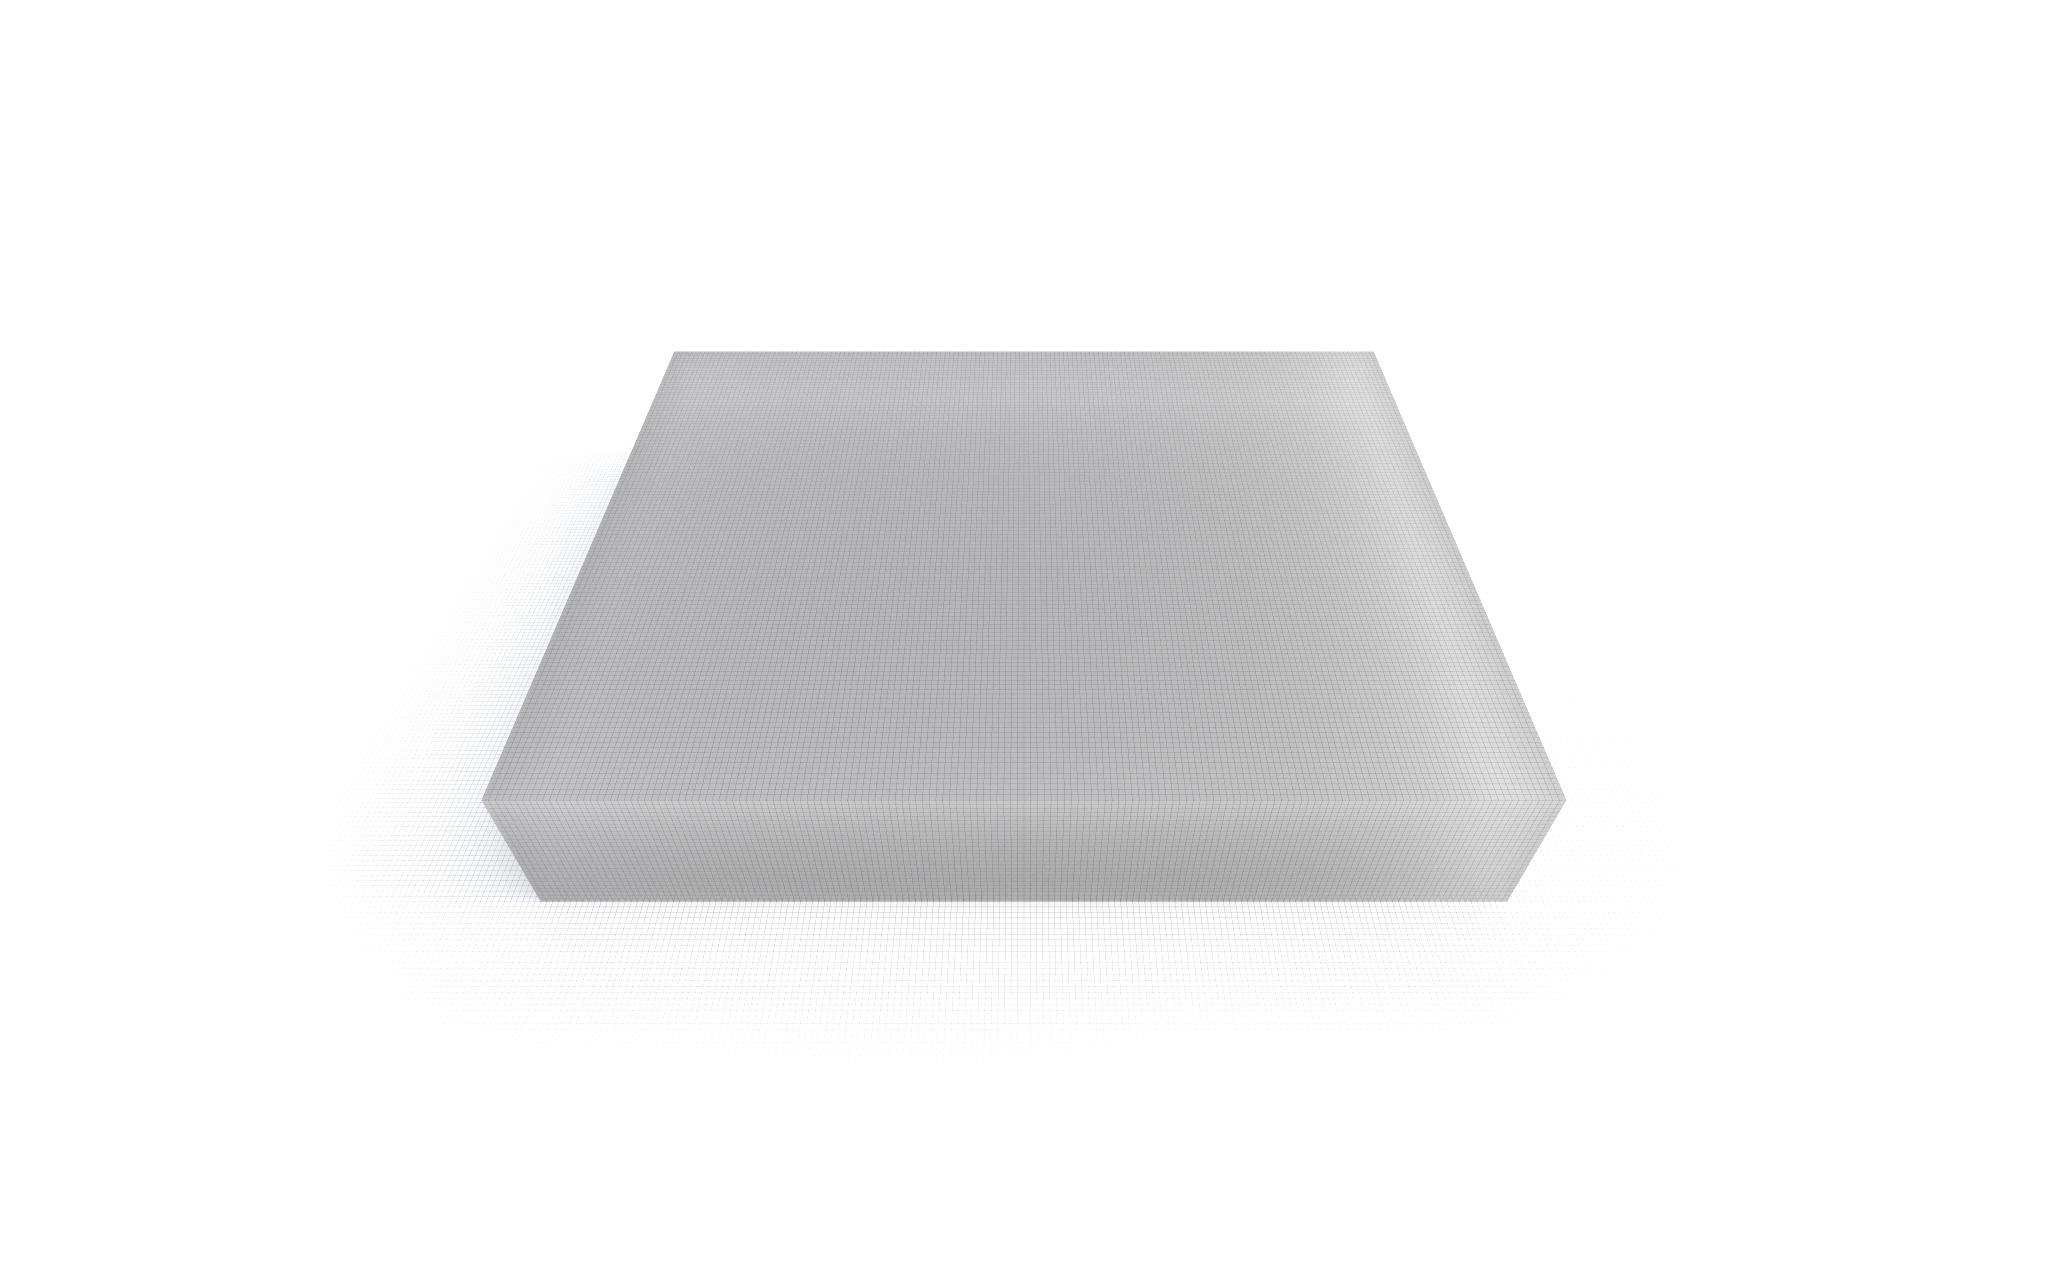
\includegraphics[trim=512 192 360 192, width=\textwidth]{figures/bbox_cam2_2048x1256_2048s-alpha.png}
            }
            \only<3>{
                \vspace{0.5em}
                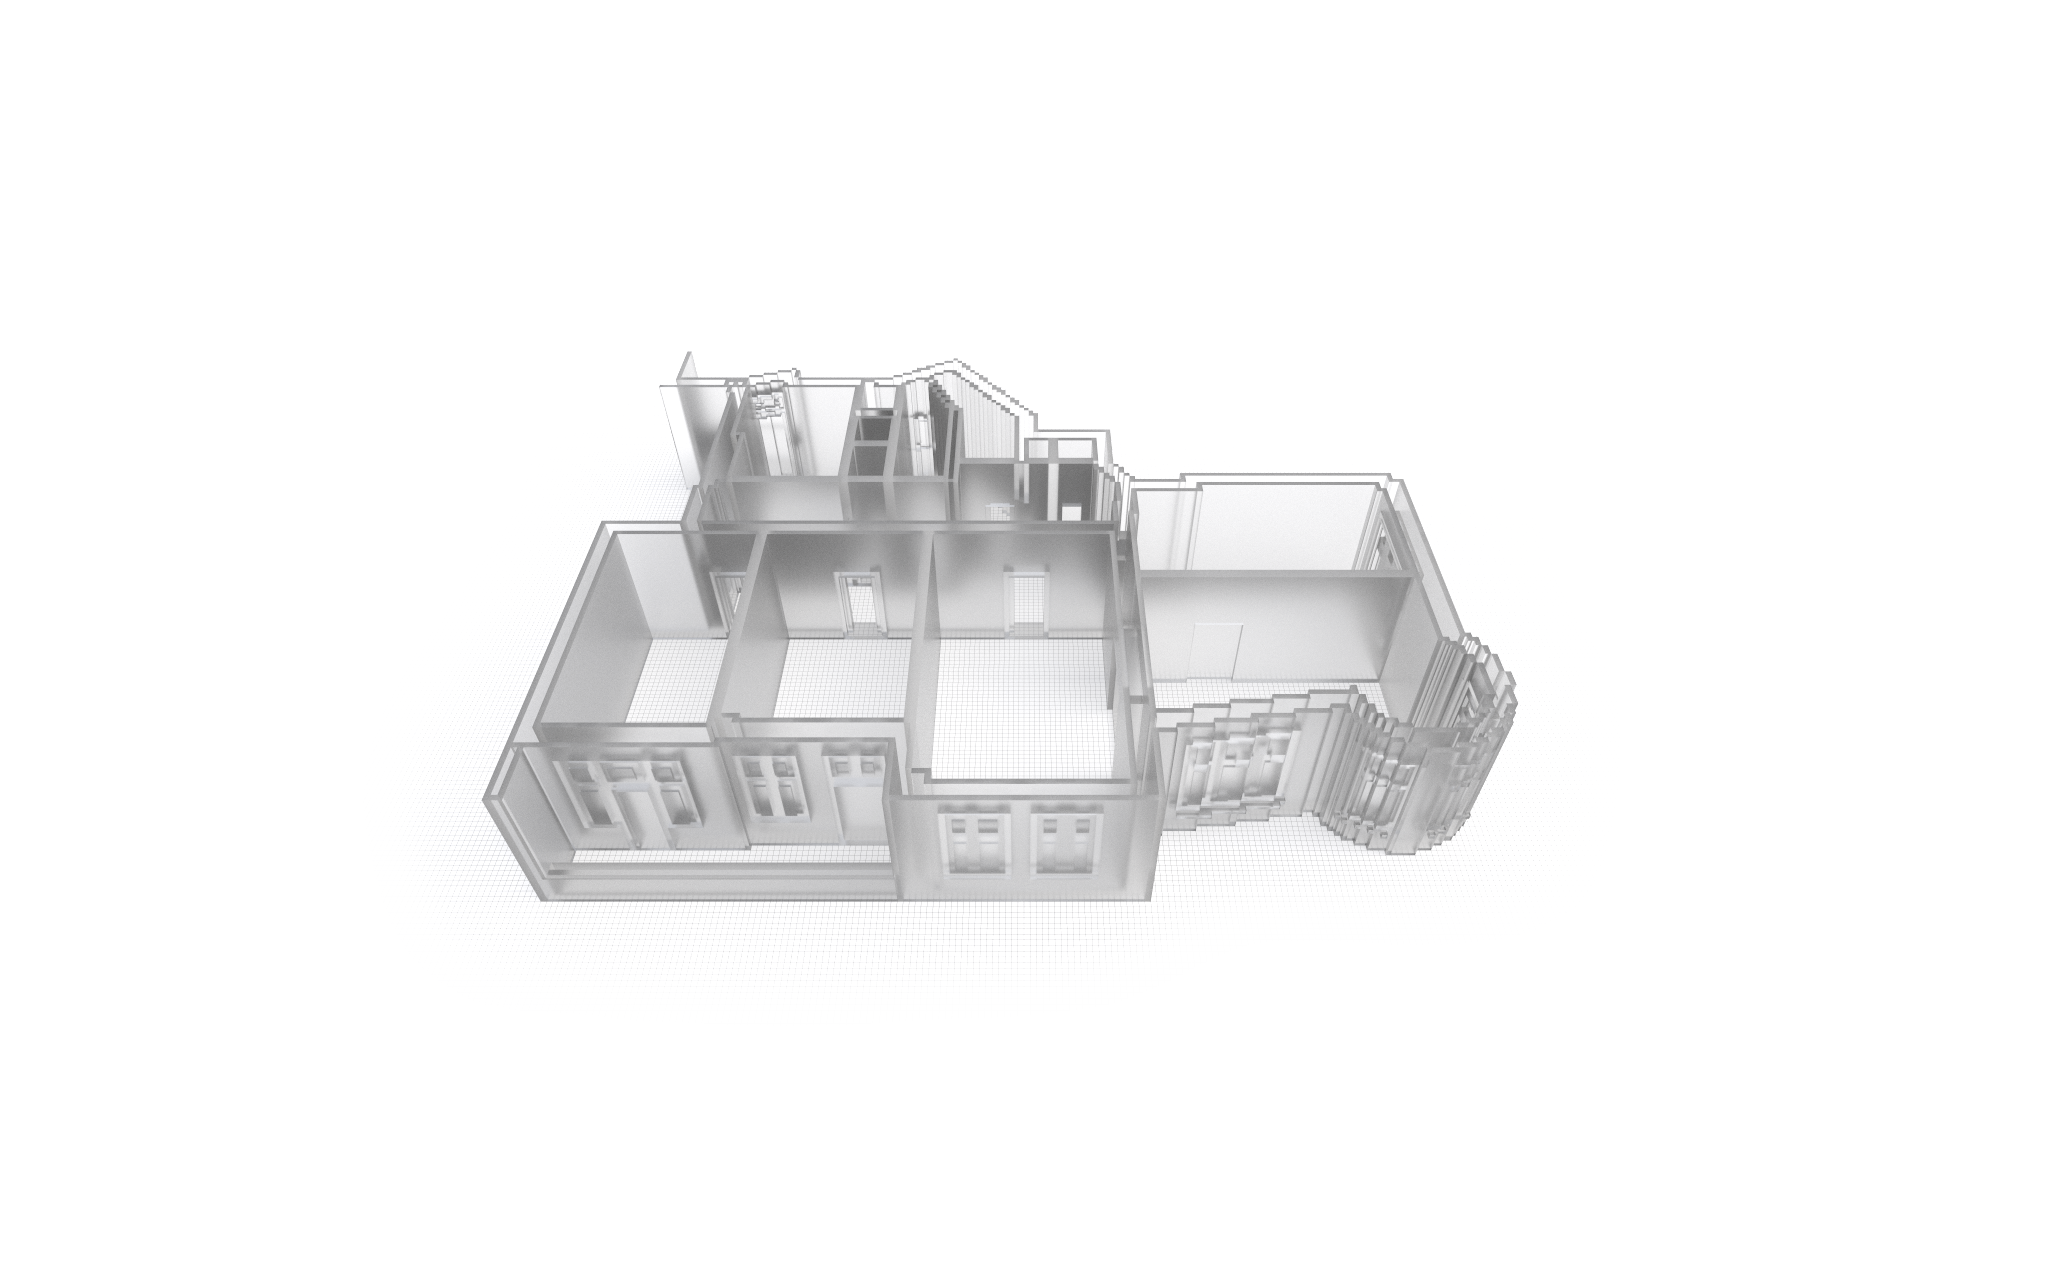
\includegraphics[trim=512 192 360 192, width=\textwidth]{figures/boundaries_cam2_2048x1256_2048s-alpha.png}
            }
            \only<4>{\vspace{0.5em}
                \begin{tikzpicture}[spy using outlines={white, rectangle, magnification=3.0, size=88, line width=2.0pt, connect spies, every spy on node/.append style={line width=1.0pt}},inner sep=0pt, outer sep=0pt]
                    \node[anchor=west](step4) at (0,0) {%
                        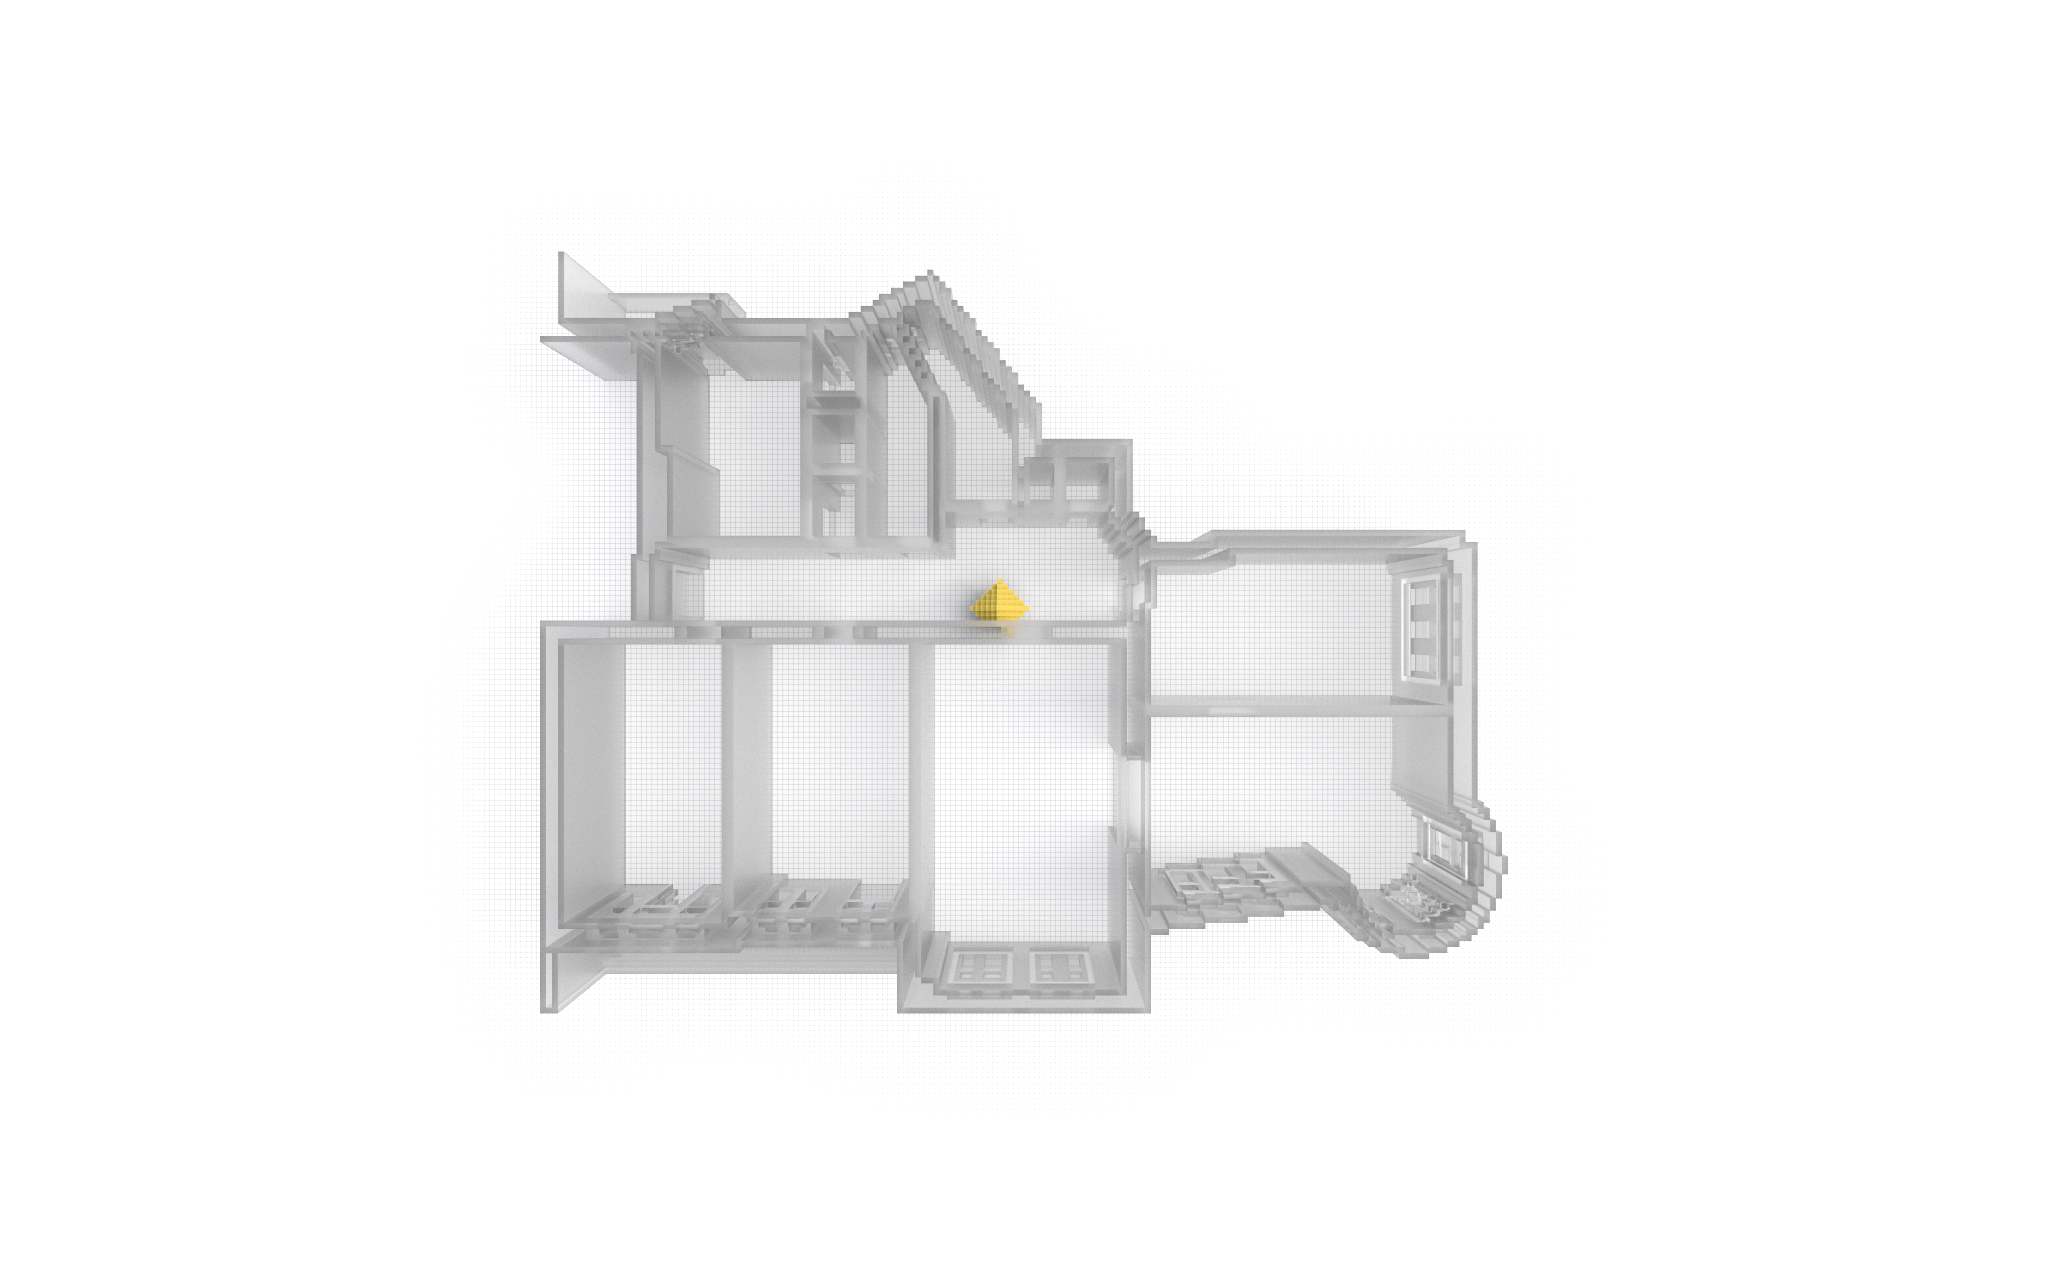
\includegraphics[trim=512 192 360 192,width=\textwidth]{figures/step1_cam1_2048x1256_2048s-alpha.png}};%
                    \spy [white] on ($(step4.center)+(-0.7, +0.15)$) in node at ($(+2.35, +1.5)+(step4.center)$);
              \end{tikzpicture}
            }
            \only<5>{
                \vspace{0.5em}
                \begin{tikzpicture}[spy using outlines={white, rectangle, magnification=3.0, size=88, line width=2.0pt, connect spies, every spy on node/.append style={line width=1.0pt}},inner sep=0pt, outer sep=0pt]
                    \node[anchor=west](step5) at (0,0) {%
                        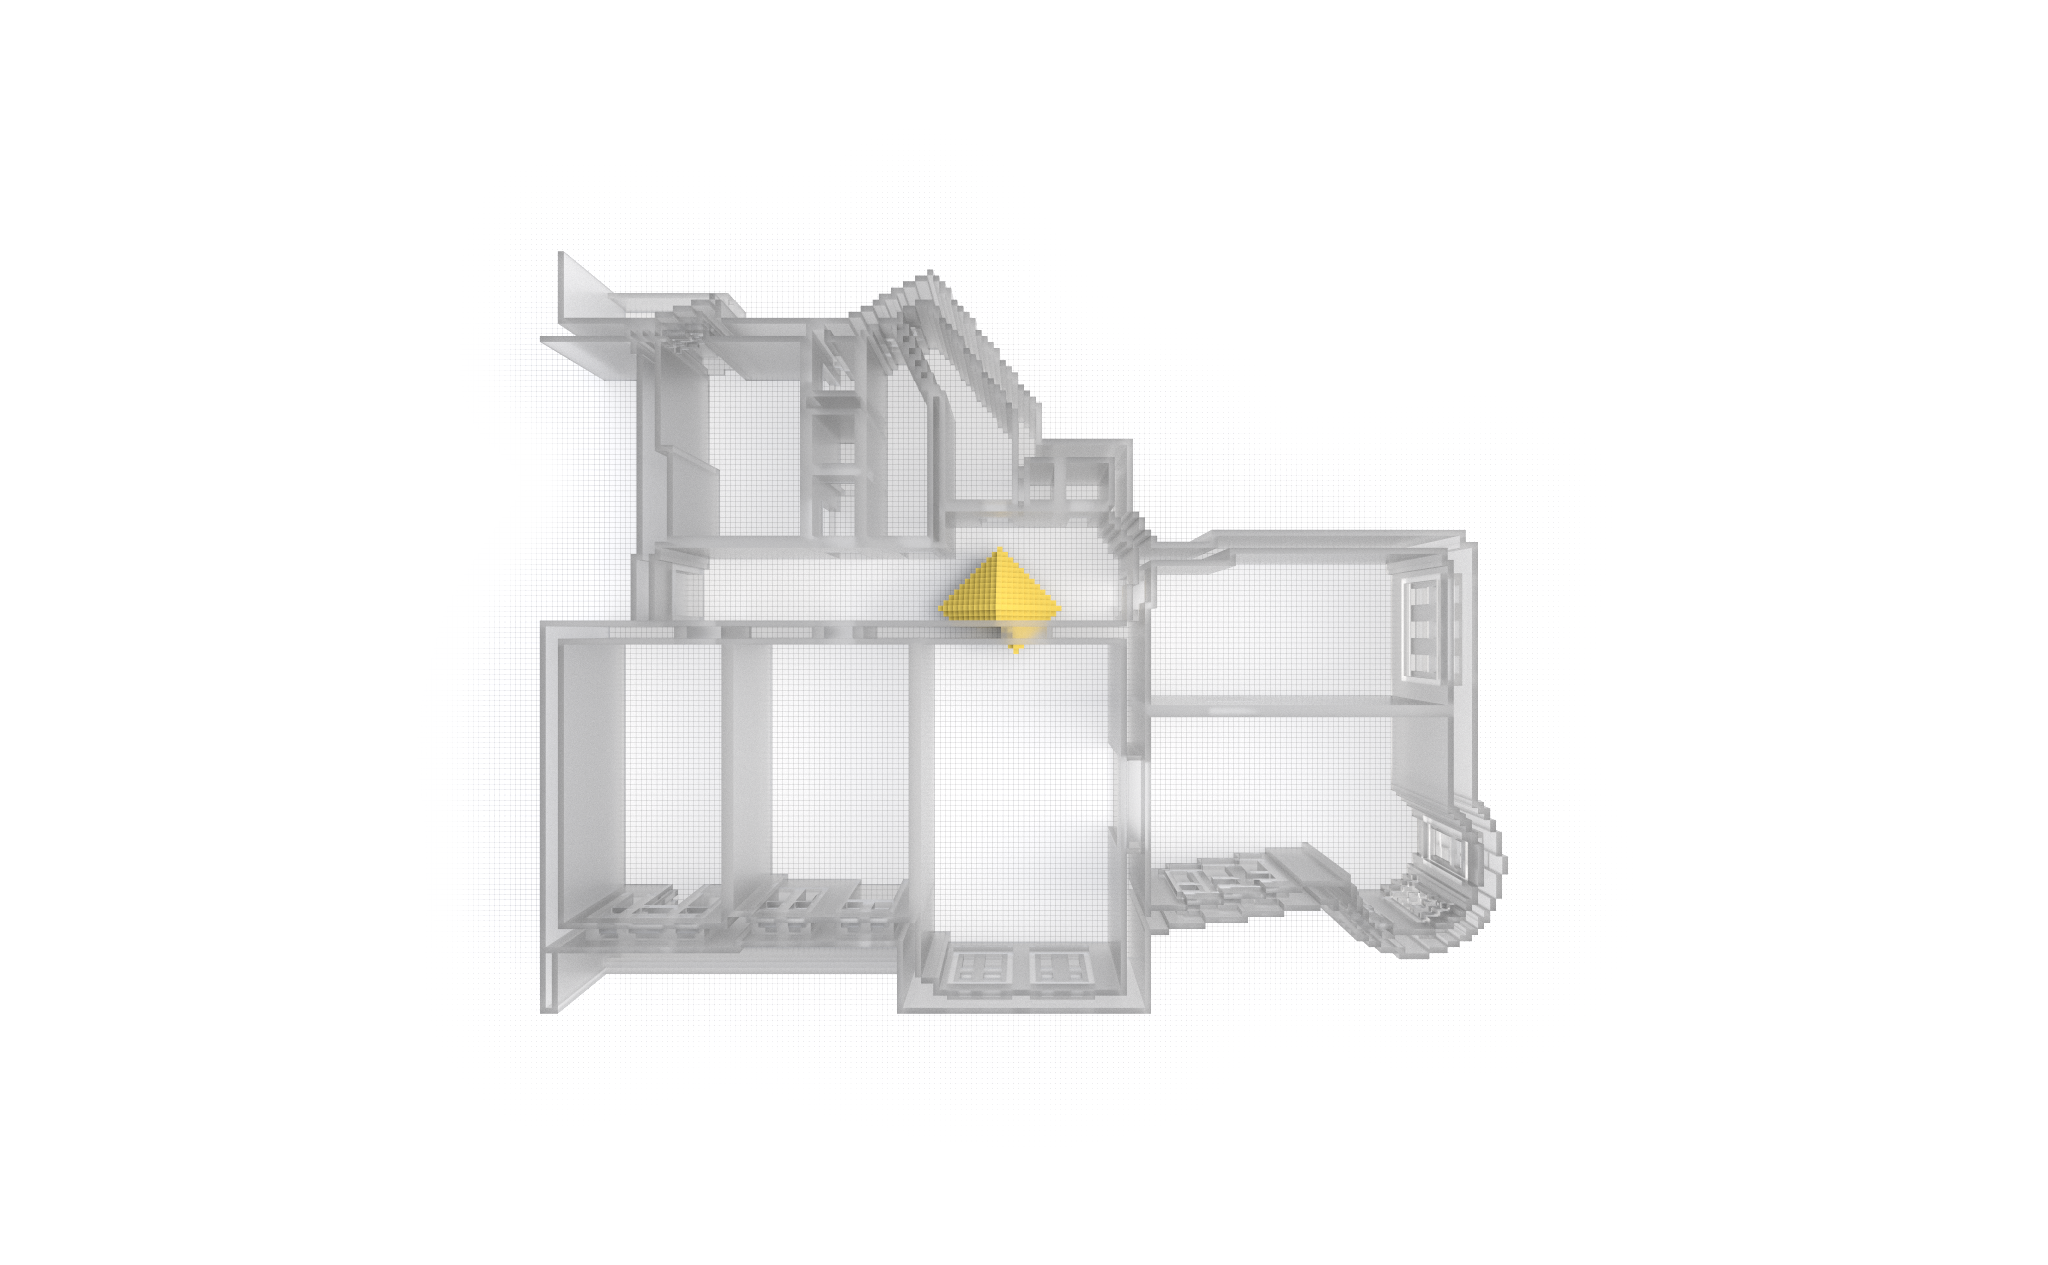
\includegraphics[trim=512 192 360 192,width=\textwidth]{figures/step1-5_cam1_2048x1256_2048s-alpha.png}};%
                    \spy [white] on ($(step5.center)+(-0.7, +0.15)$) in node at ($(+2.35, +1.5)+(step5.center)$);
                \end{tikzpicture}
            }
            \only<6>{
                \vspace{0.5em}
                \begin{tikzpicture}[spy using outlines={white, rectangle, magnification=3.0, size=88, line width=2.0pt, connect spies, every spy on node/.append style={line width=1.0pt}},inner sep=0pt, outer sep=0pt]
                    \node[anchor=west](step6) at (0,0) {%
                        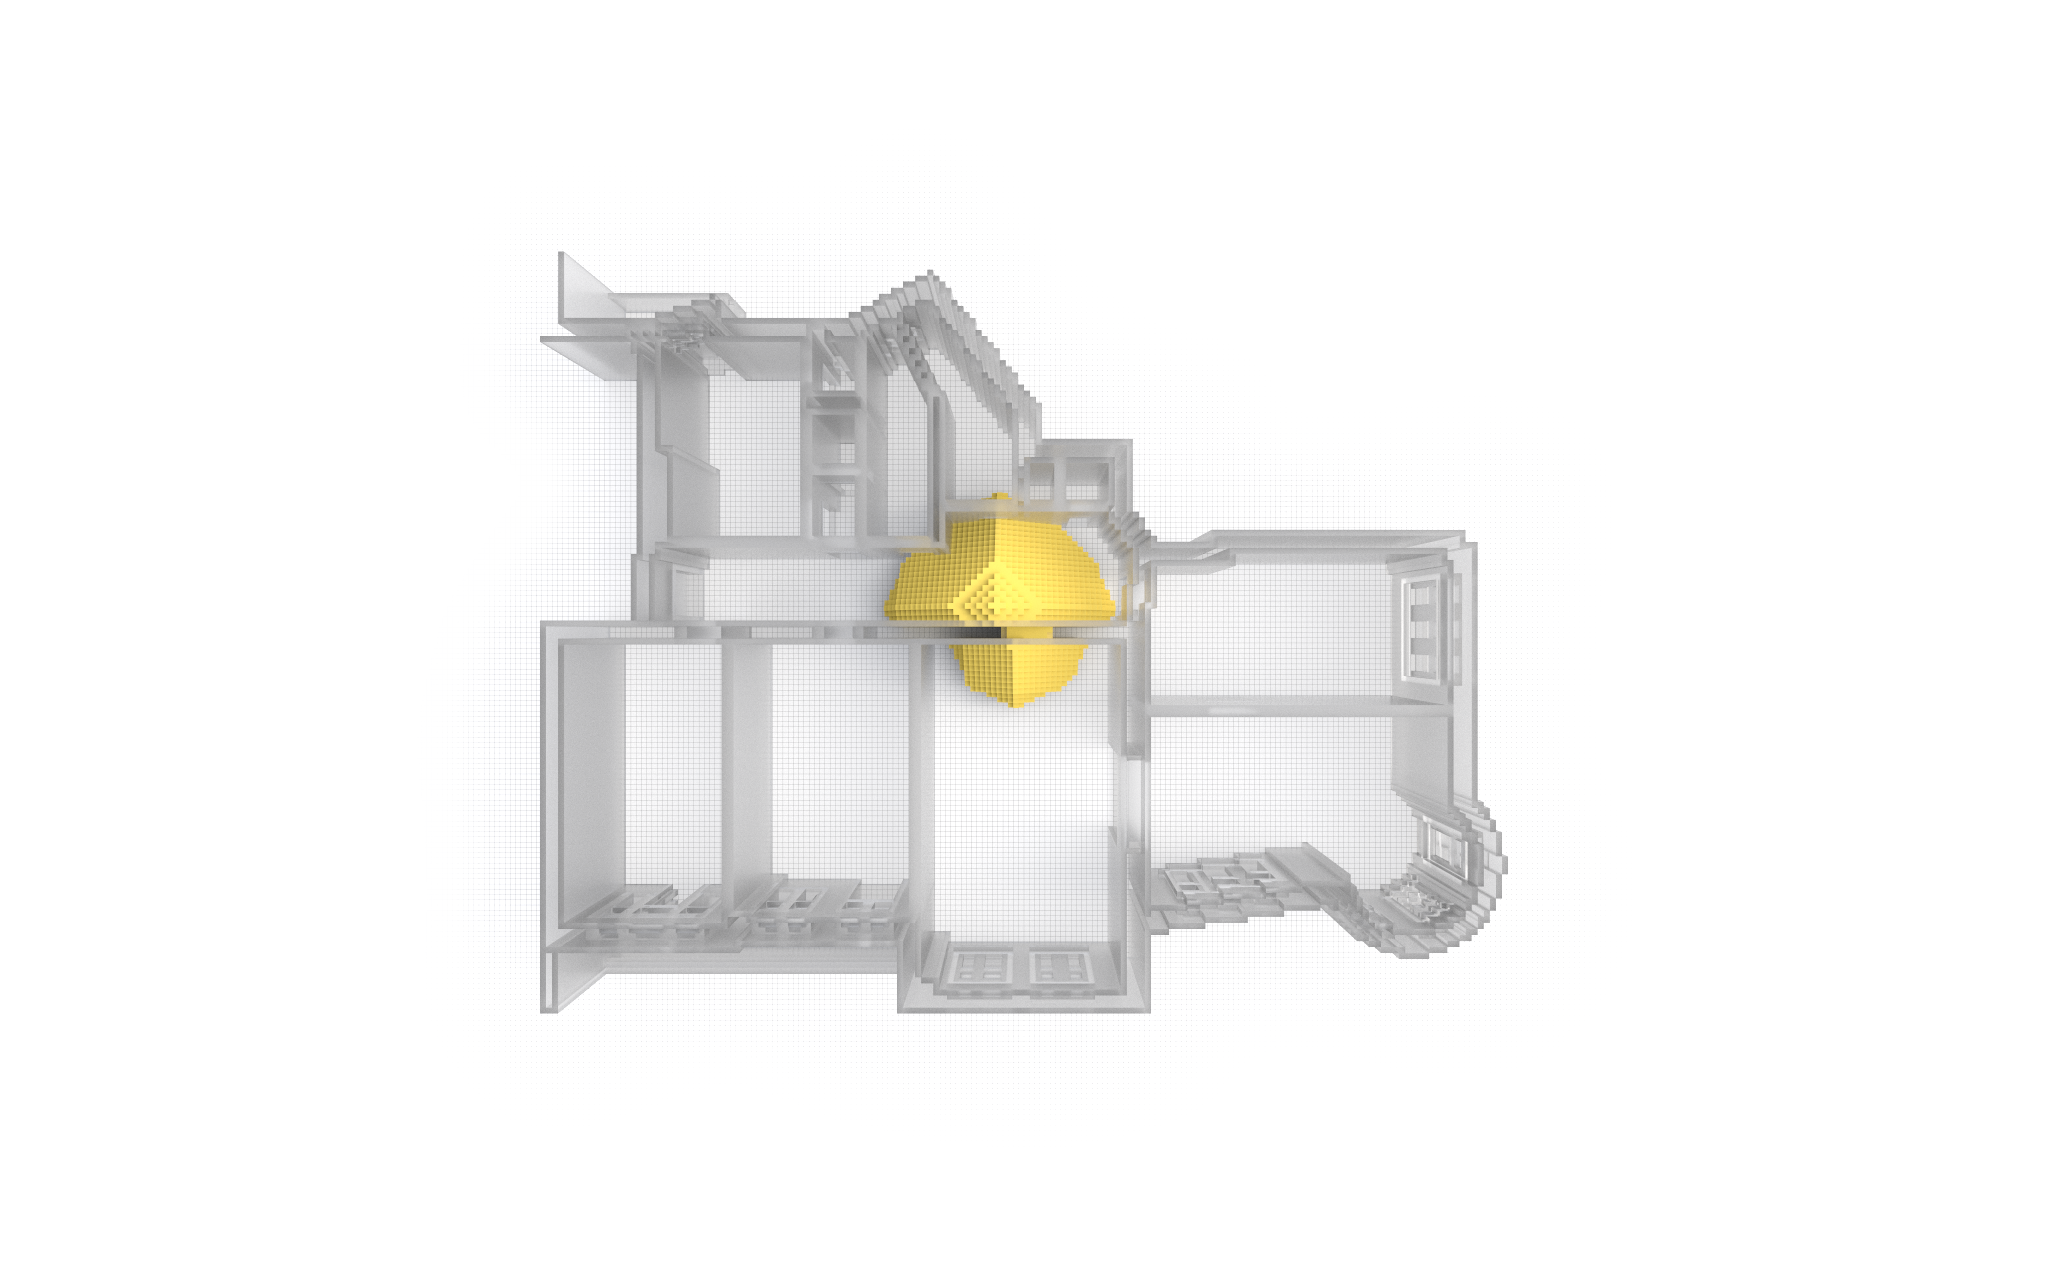
\includegraphics[trim=512 192 360 192,width=\textwidth]{figures/step2_cam1_2048x1256_2048s-alpha.png}};%
                    \spy [white] on ($(step6.center)+(-0.7, +0.15)$) in node at ($(+2.35, +1.5)+(step6.center)$);
                \end{tikzpicture}
            }

        \end{column}
    \end{columns}

\end{frame}

\begin{frame}[t]{System Details\enspace{}|\enspace{}\textbf{Per-Sensor Distance Map Computation}}

    Due to limitations in WebAPIs regarding 3D texture loading: Encoded in two 8-bit, stacked 2D textures.

    \vspace{-0.5em}
    \begin{columns}[T]

        \begin{column}{0.47\textwidth}
           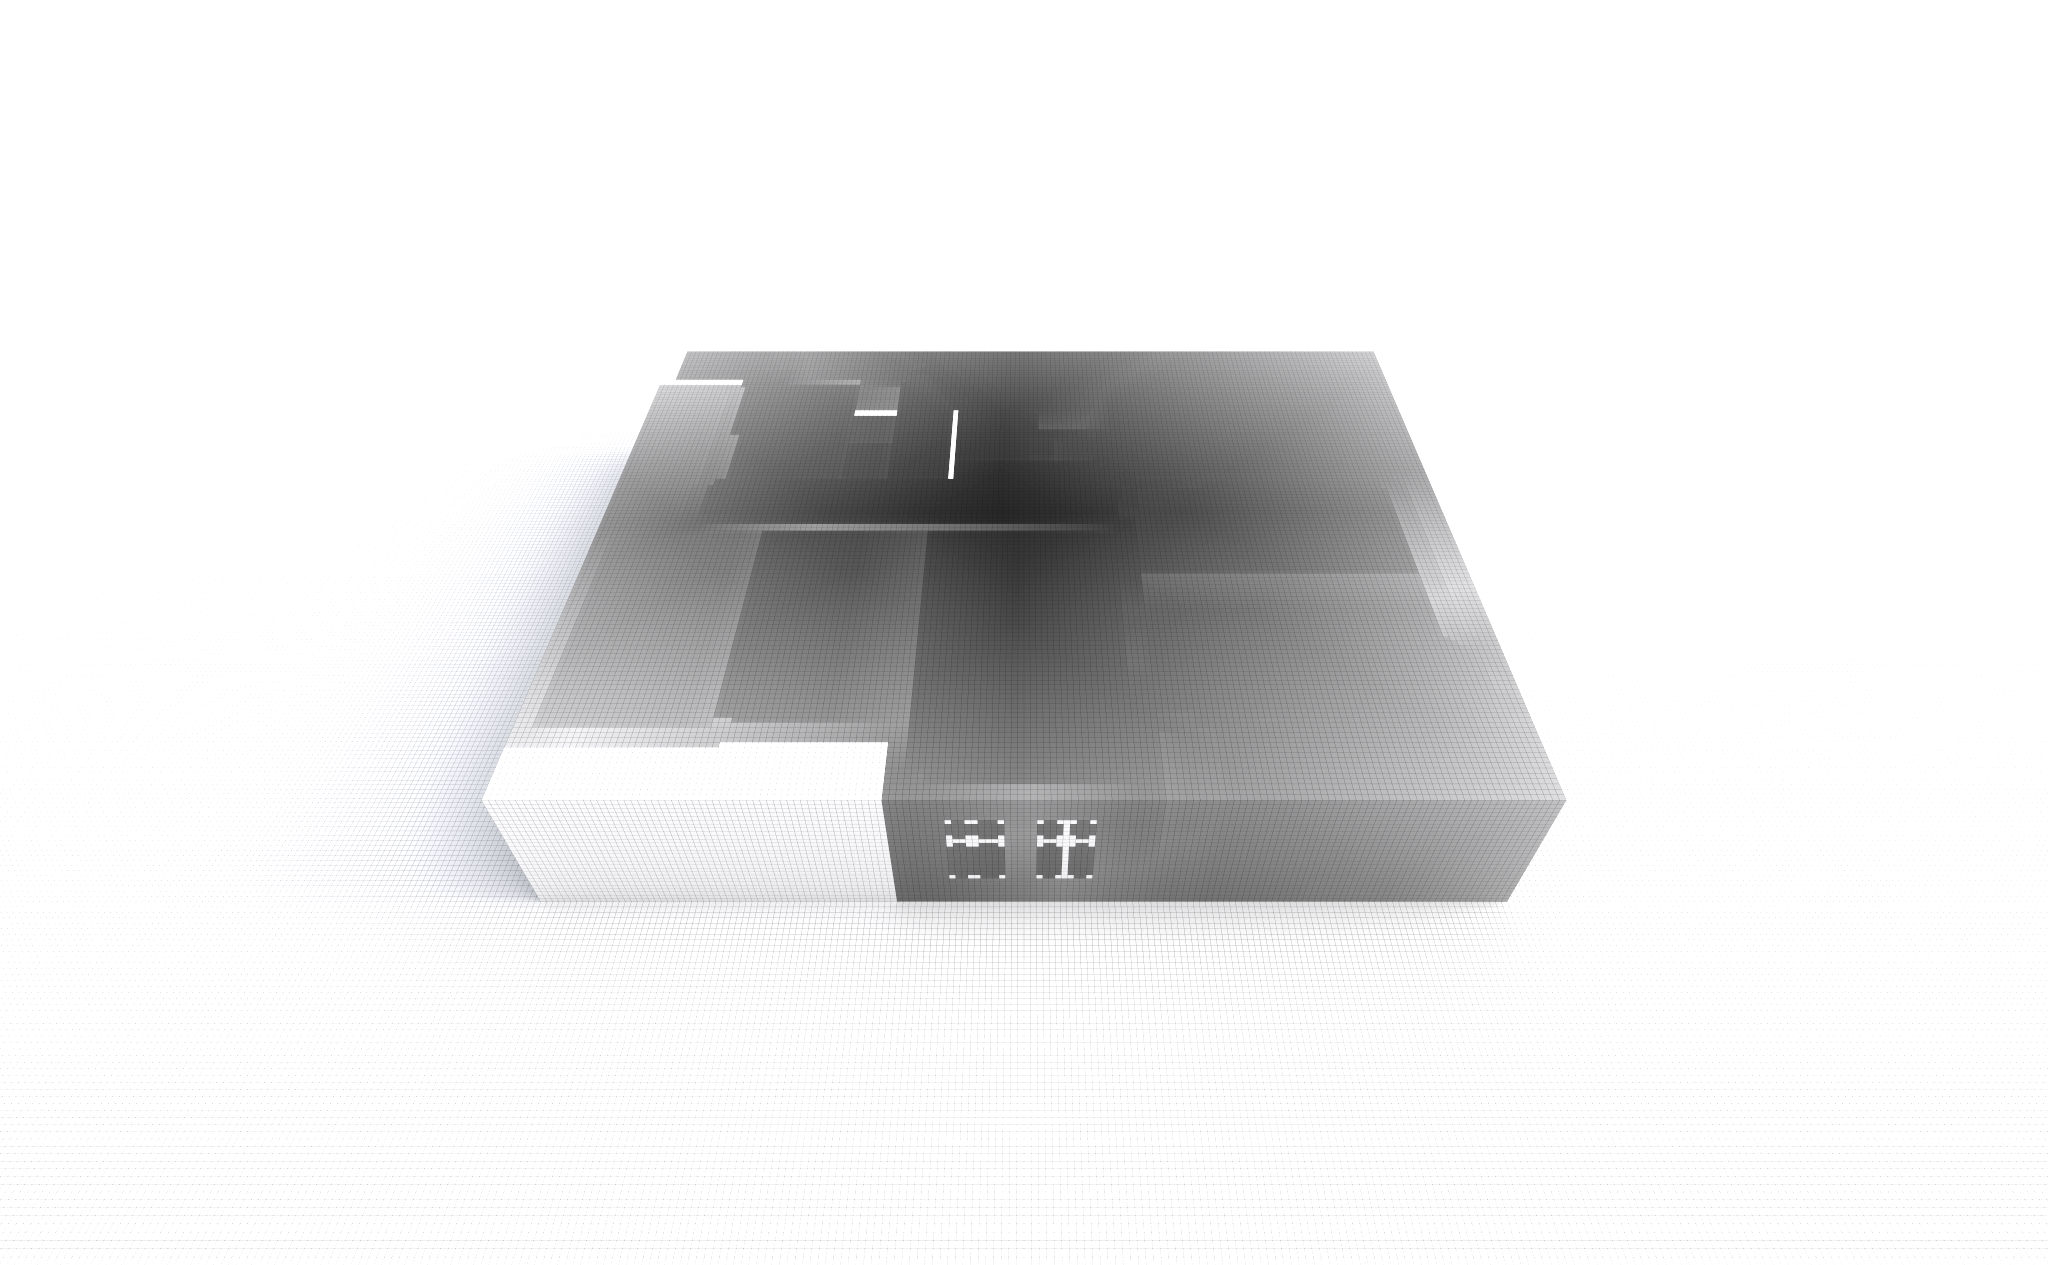
\includegraphics[trim=360 140 360 140, clip,width=\textwidth]{figures/3d-texture_cam2_2048x1256_2048s.png}
        \end{column}
        
        \begin{column}{0.47\textwidth}
            \bigskip
            \bigskip
            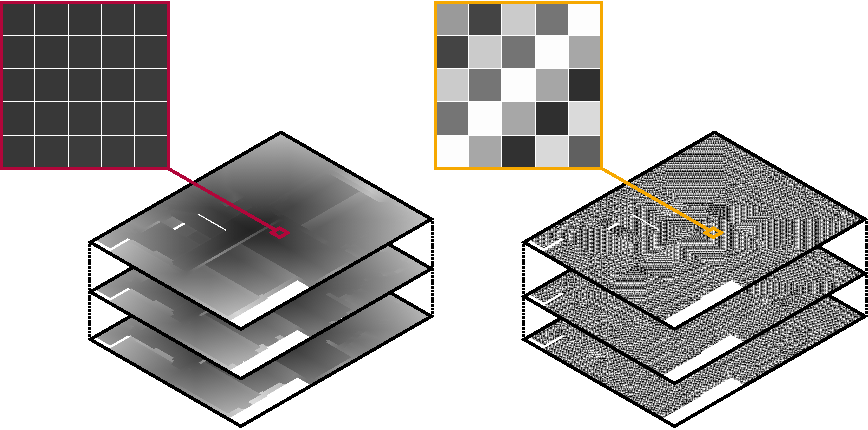
\includegraphics[width=\textwidth]{figures/stacked-bit-separated-3d-distance-maps__eurovis_no-labels.pdf}
        \end{column}

    \end{columns}
    
    \vspace{-0.5em}
    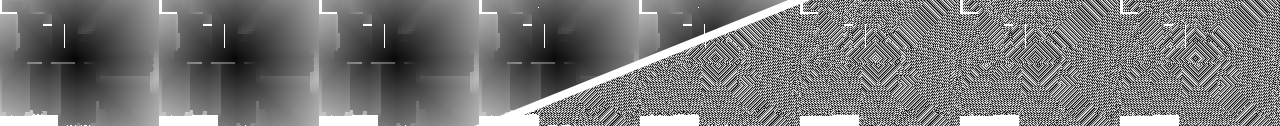
\includegraphics[width=\textwidth]{figures/sensor_348_cropped_mixed.png}

\end{frame}

\begin{frame}[t]{System Details\enspace{}|\enspace{}\textbf{Labeling Algorithm}}

    \begin{columns}[T]
        \begin{column}{0.372\textwidth}

            \smallskip
            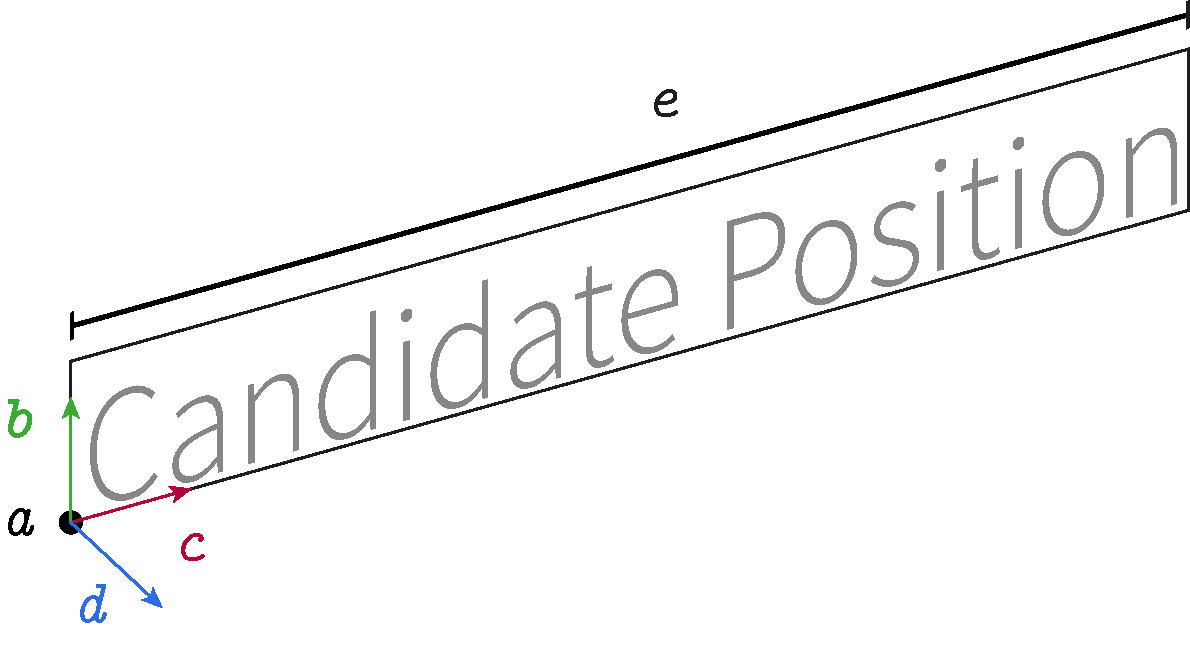
\includegraphics[width=1.0\textwidth]{figures/labeling-algorithm_label-attributes-v3_texttt.pdf}
            \smallskip

            \textbf{Attributes used for the algorithm:}
            \begin{itemize}\setlength\itemsep{0pt}
                \item [\itshape\texttt{\color{black}a}]
                    candidate's anchor point,%
                \item [\itshape\texttt{\color{custom@green}b}]
                    upwards-facing vector,
                \item [\itshape\texttt{\color{custom@red}c}]
                    running direction vector,
                \item [\itshape\texttt{\color{eurovis@blue}d}]
                    forward-facing normal vector,
                \item [\itshape\texttt{\color{custom@gray}e}]
                    maximum available length. %
            \end{itemize}

        \end{column}

        \begin{column}{0.568\textwidth}

            \begin{figure}
                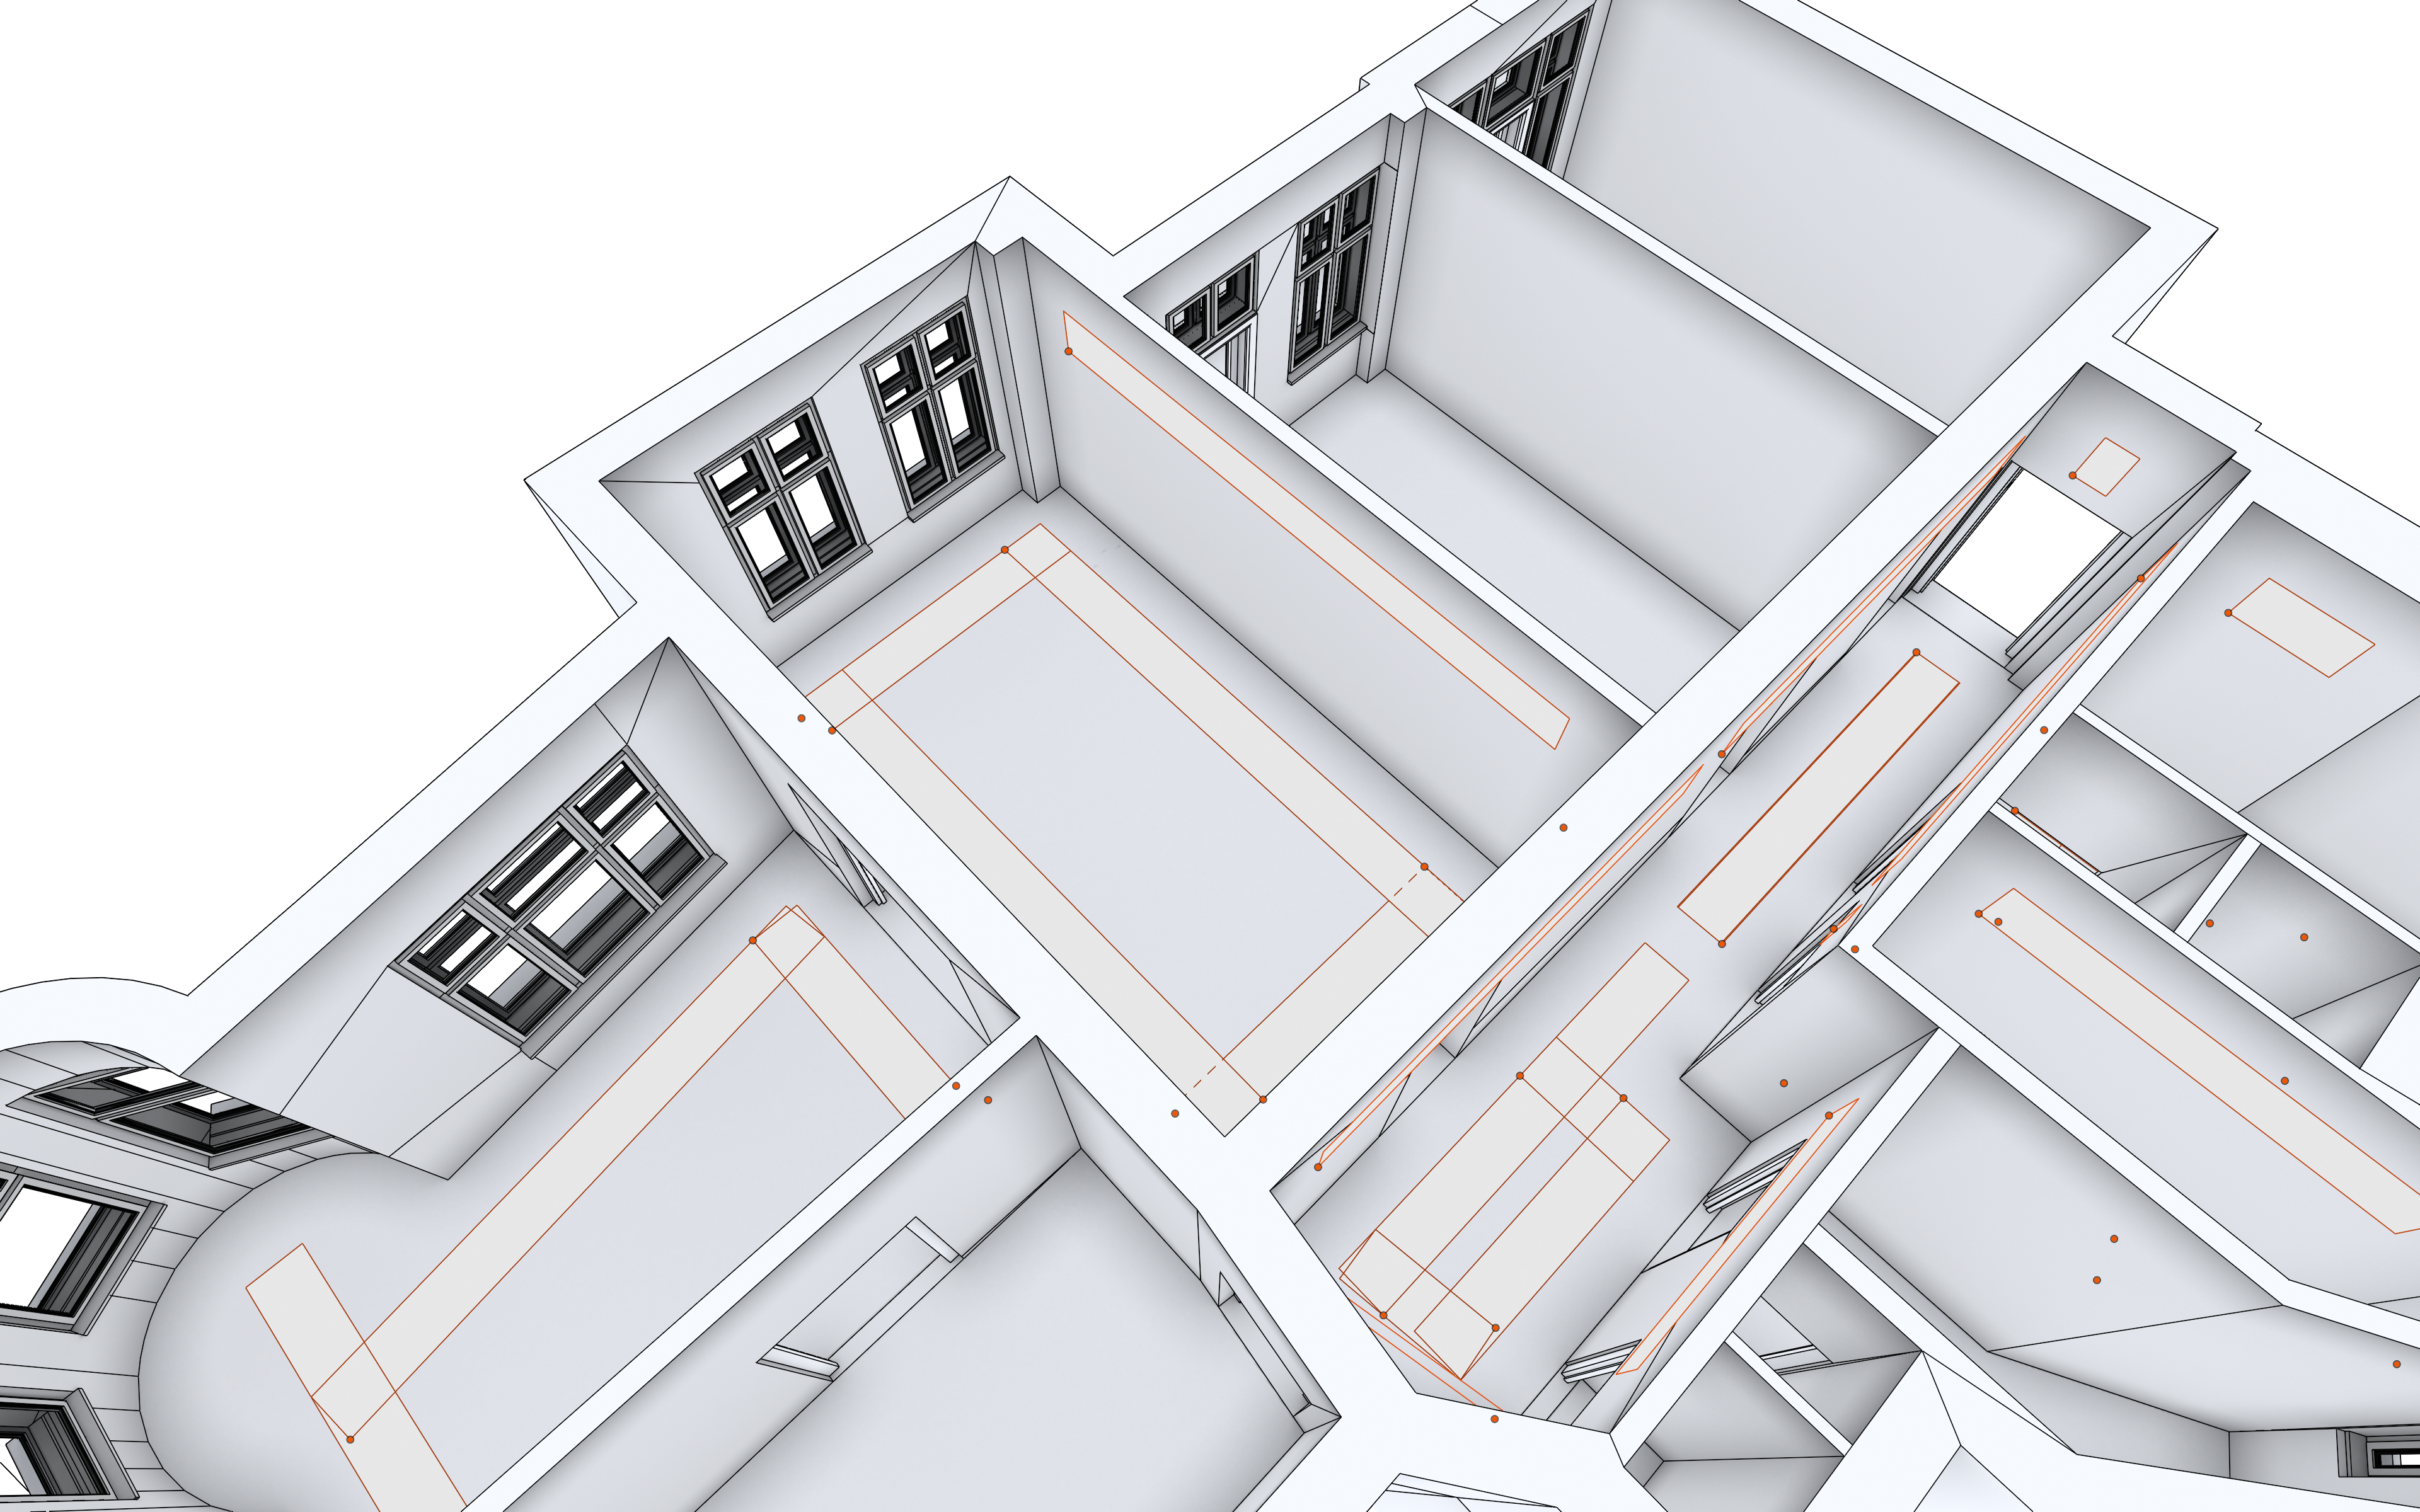
\includegraphics[width=1.0\textwidth]{figures/labelling-scene__blank.png}
                \caption*{Labeling candidates are currently created manually but could be precomputed in future work.}
            \end{figure}

        \end{column}
    \end{columns}

\end{frame}

\begin{frame}[t]{System Details\enspace{}|\enspace{}\textbf{Labeling Algorithm}}

    \begin{columns}[T]
        \begin{column}{0.372\textwidth}
            
            \textbf{Filtering rules:}
        
            \begin{enumerate}
                \item Label faces camera
                    \only<1>{\\ \vspace{0.2em} \textit{Based on dot product between forward-facing normal vector~\texttt{\color{eurovis@blue}d}\hspace{.2em} and vector from camera eye to label’s world coordinate \texttt{\color{black}a}}
                }
               \only<2->{
                    \item Label is inside visible viewport \only<2>{\\ \smallskip
                     \textit{Computed by transforming anchor point~\texttt{\color{black}a}\hspace{.2em} to normalized device coordinates (NDC)}}
                }
                \only<3->{
                    \item Label is not upside down \only<3>{\\ \smallskip
                    \textit{Calculated by transforming upwards-facing vector~\texttt{\color{custom@green}b}\hspace{.2em} to NDC and calculating dot product with screen’s upwards-facing vector}}
                }
                \only<4->{
                    \item Label is not behind obstacle \only<4>{\\ \smallskip
                    \textit{Done via lookup of transformed anchor point position~\texttt{\color{black}a}\hspace{.2em} (in NDC) in depth G-buffer and subsequent transformation to world coordinates}}
                }
            \end{enumerate}

            \only<5->{
                \vspace{0.5em}
                If multiple candidate positions pass filtering: Metric-driven comparison
            }
        \end{column}
        \begin{column}{0.568\textwidth}
            \begin{figure}
                \centering
                \only<1>{
                    \begin{tikzpicture}[spy using outlines={white, rectangle, magnification=3.0, size=88, line width=2.0pt, connect spies, every spy on node/.append style={line width=1.0pt}},inner sep=0pt, outer sep=0pt]
                        \node[anchor=west](step1) at (0,0) {%
                            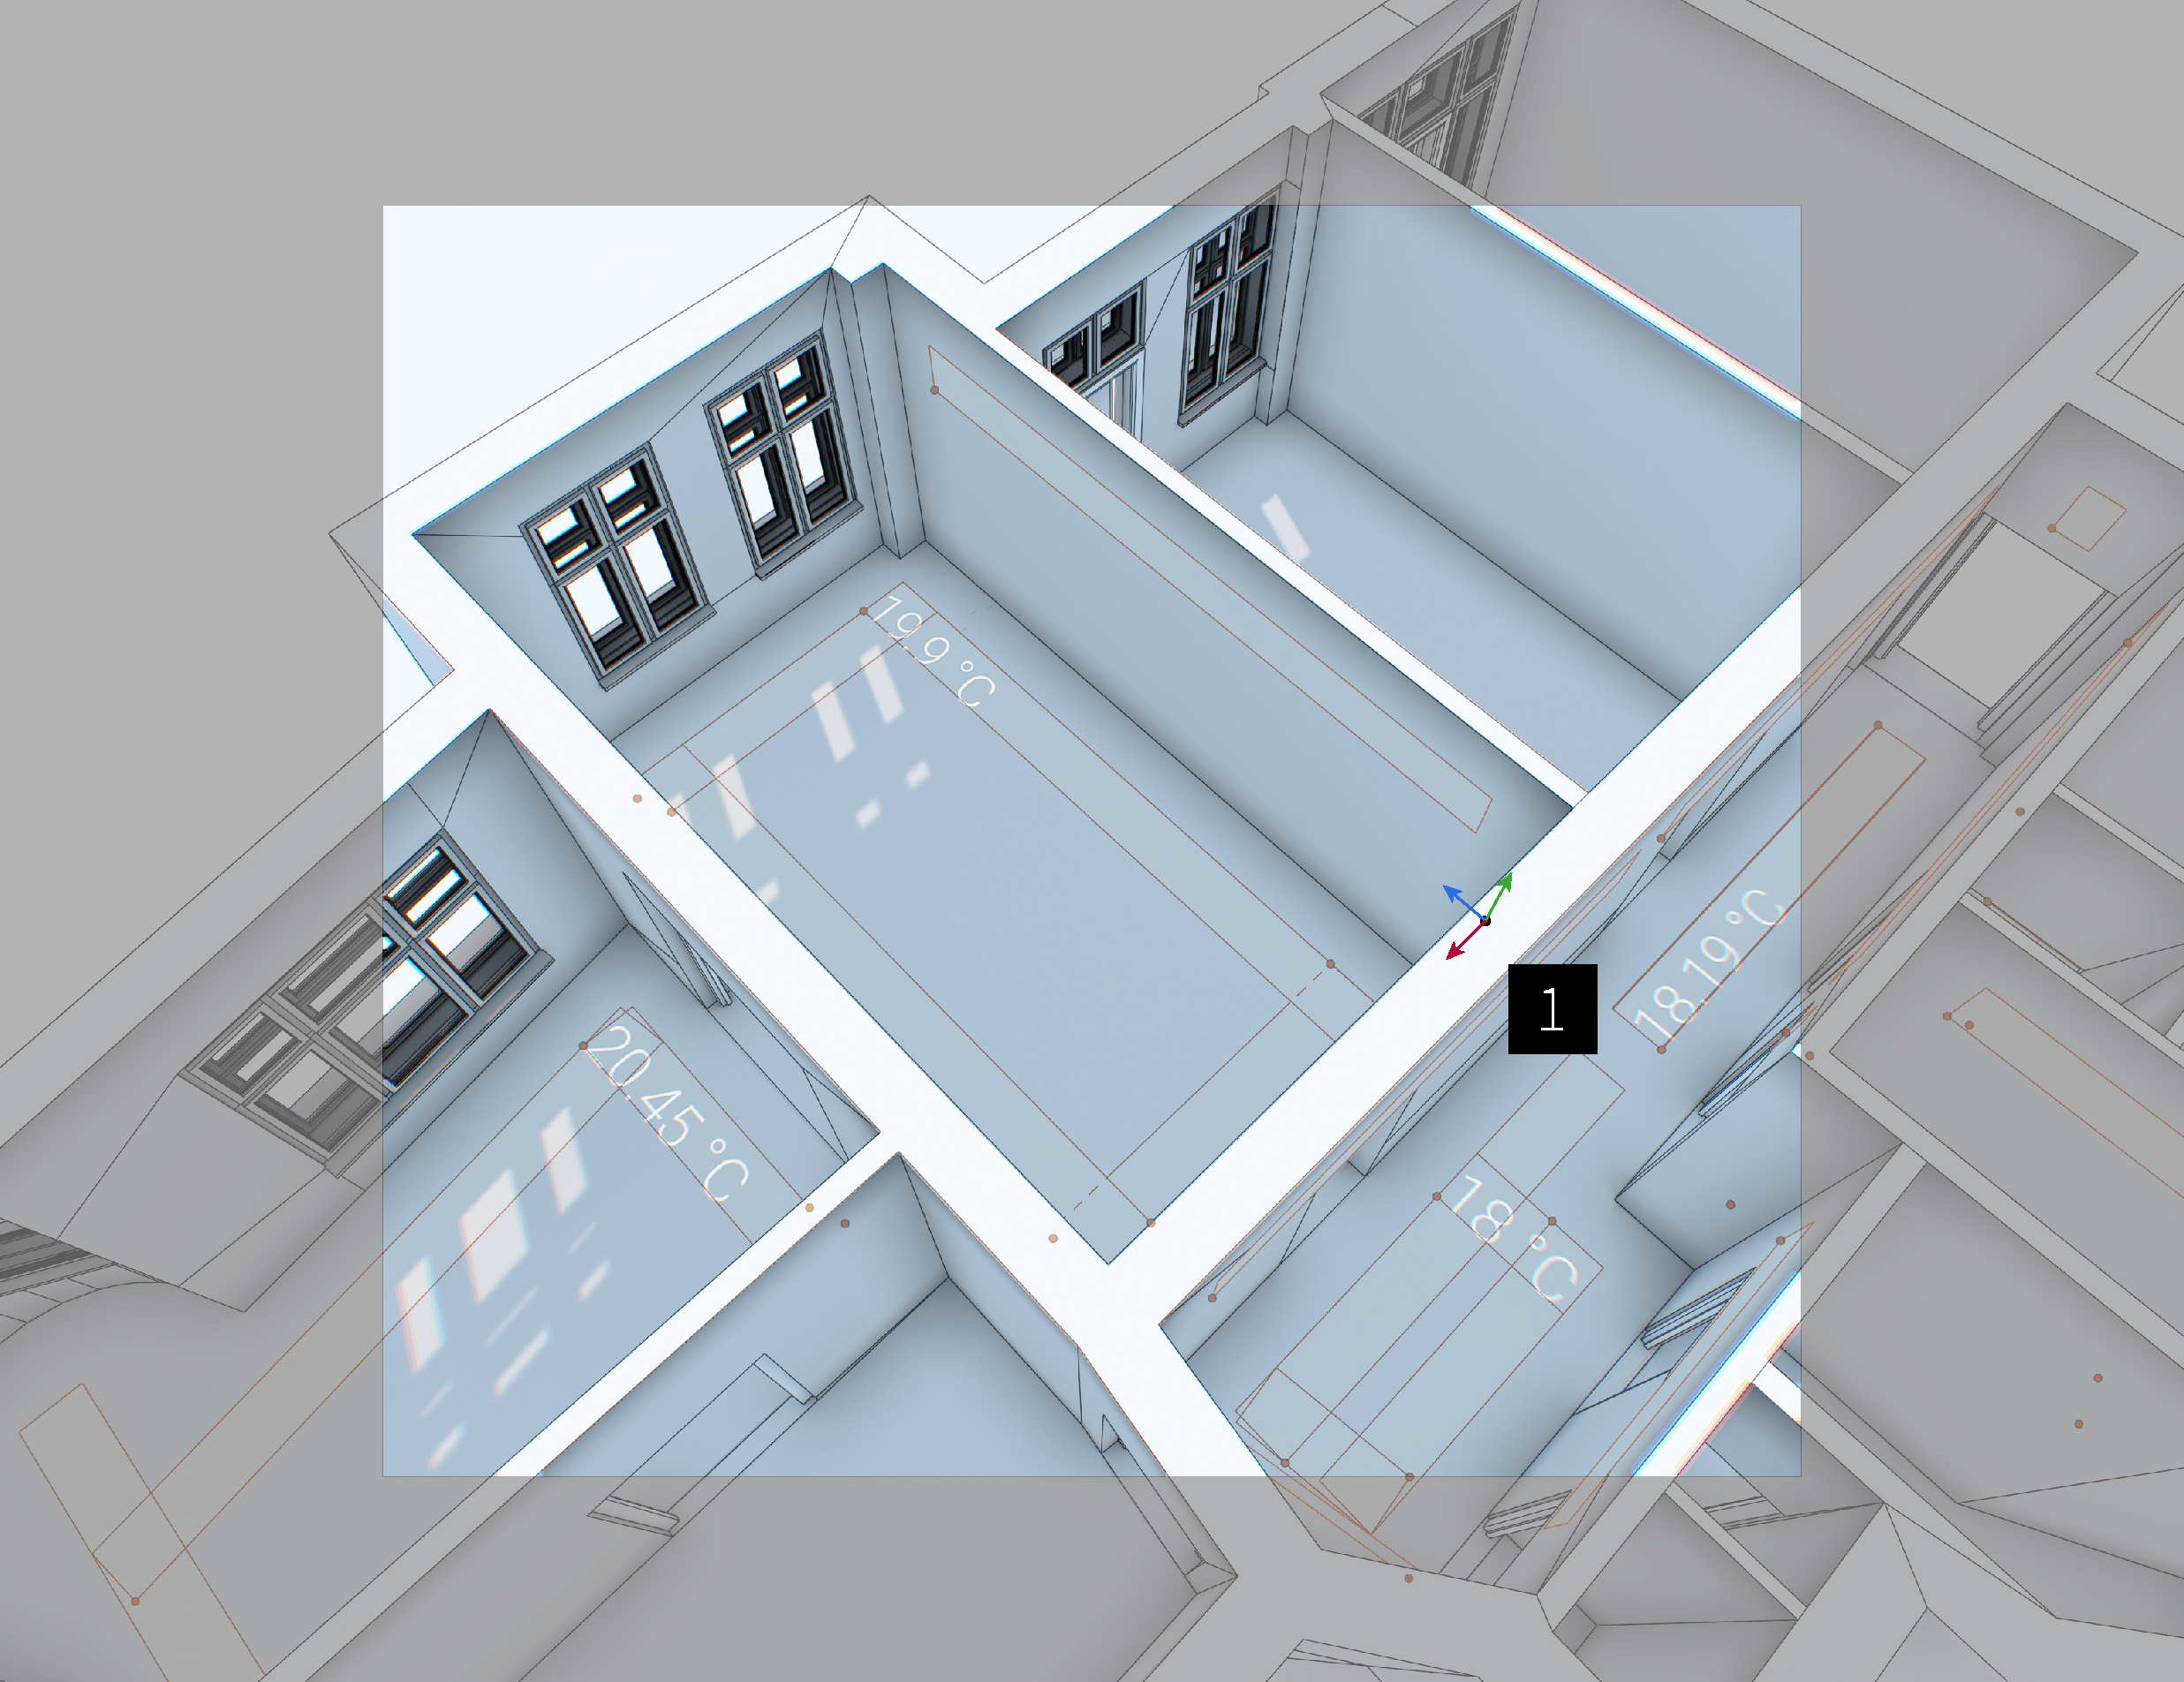
\includegraphics[width=1.0\textwidth]{figures/labelling-scene__step-1.pdf}};%
                        \spy [white] on ($(step1.center)+(+1.5, -0.4)$) in node at ($(-2.1, +1.2)+(step1.center)$);
                      \end{tikzpicture}
             }
                \only<2>{
                    \begin{tikzpicture}[spy using outlines={white, rectangle, magnification=3.0, size=88, line width=2.0pt, connect spies, every spy on node/.append style={line width=1.0pt}},inner sep=0pt, outer sep=0pt]
                        \node[anchor=west](step2) at (0,0) {%
                            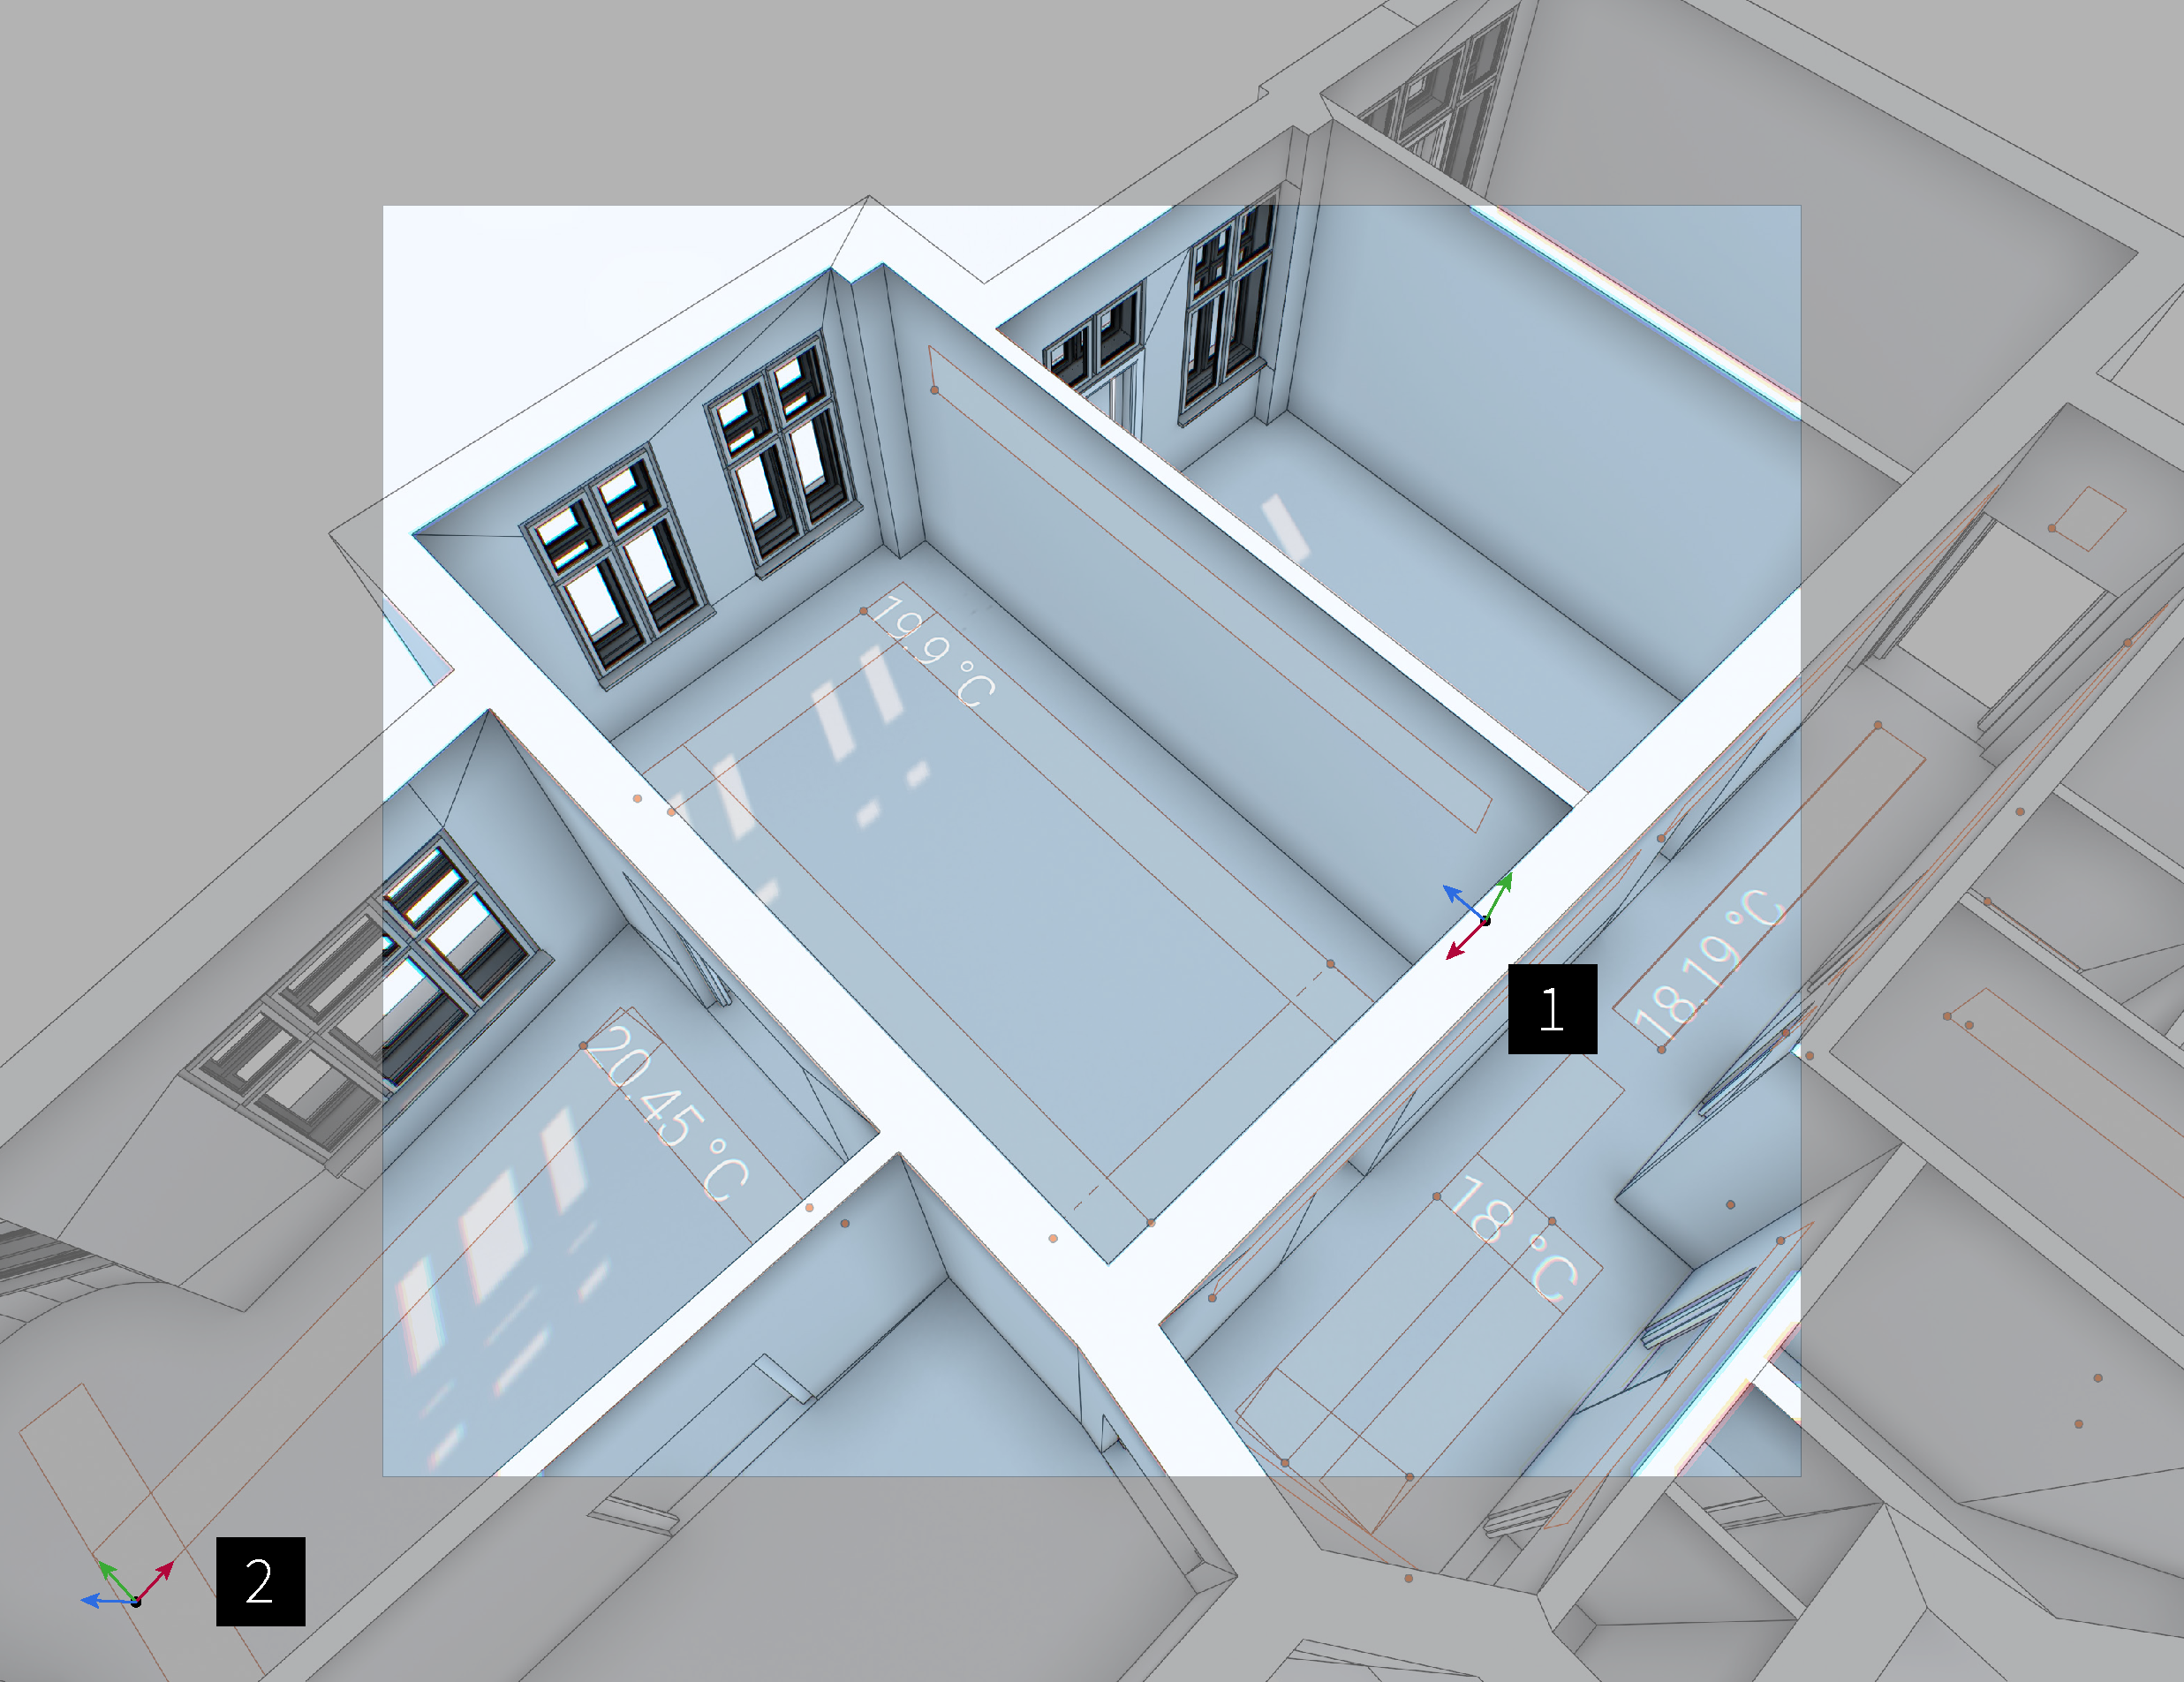
\includegraphics[width=1.0\textwidth]{figures/labelling-scene__step-2.pdf}};%
                        \spy [white] on ($(step2.center)+(-3.33, -2.55)$) in node [fill=white] at ($(+2.1, -1.2)+(step2.center)$);
                    \end{tikzpicture}
                }
                \only<3>{
                    \begin{tikzpicture}[spy using outlines={white, rectangle, magnification=3.0, size=88, line width=2.0pt, connect spies, every spy on node/.append style={line width=1.0pt}},inner sep=0pt, outer sep=0pt]
                        \node[anchor=west](step3) at (0,0) {%
                            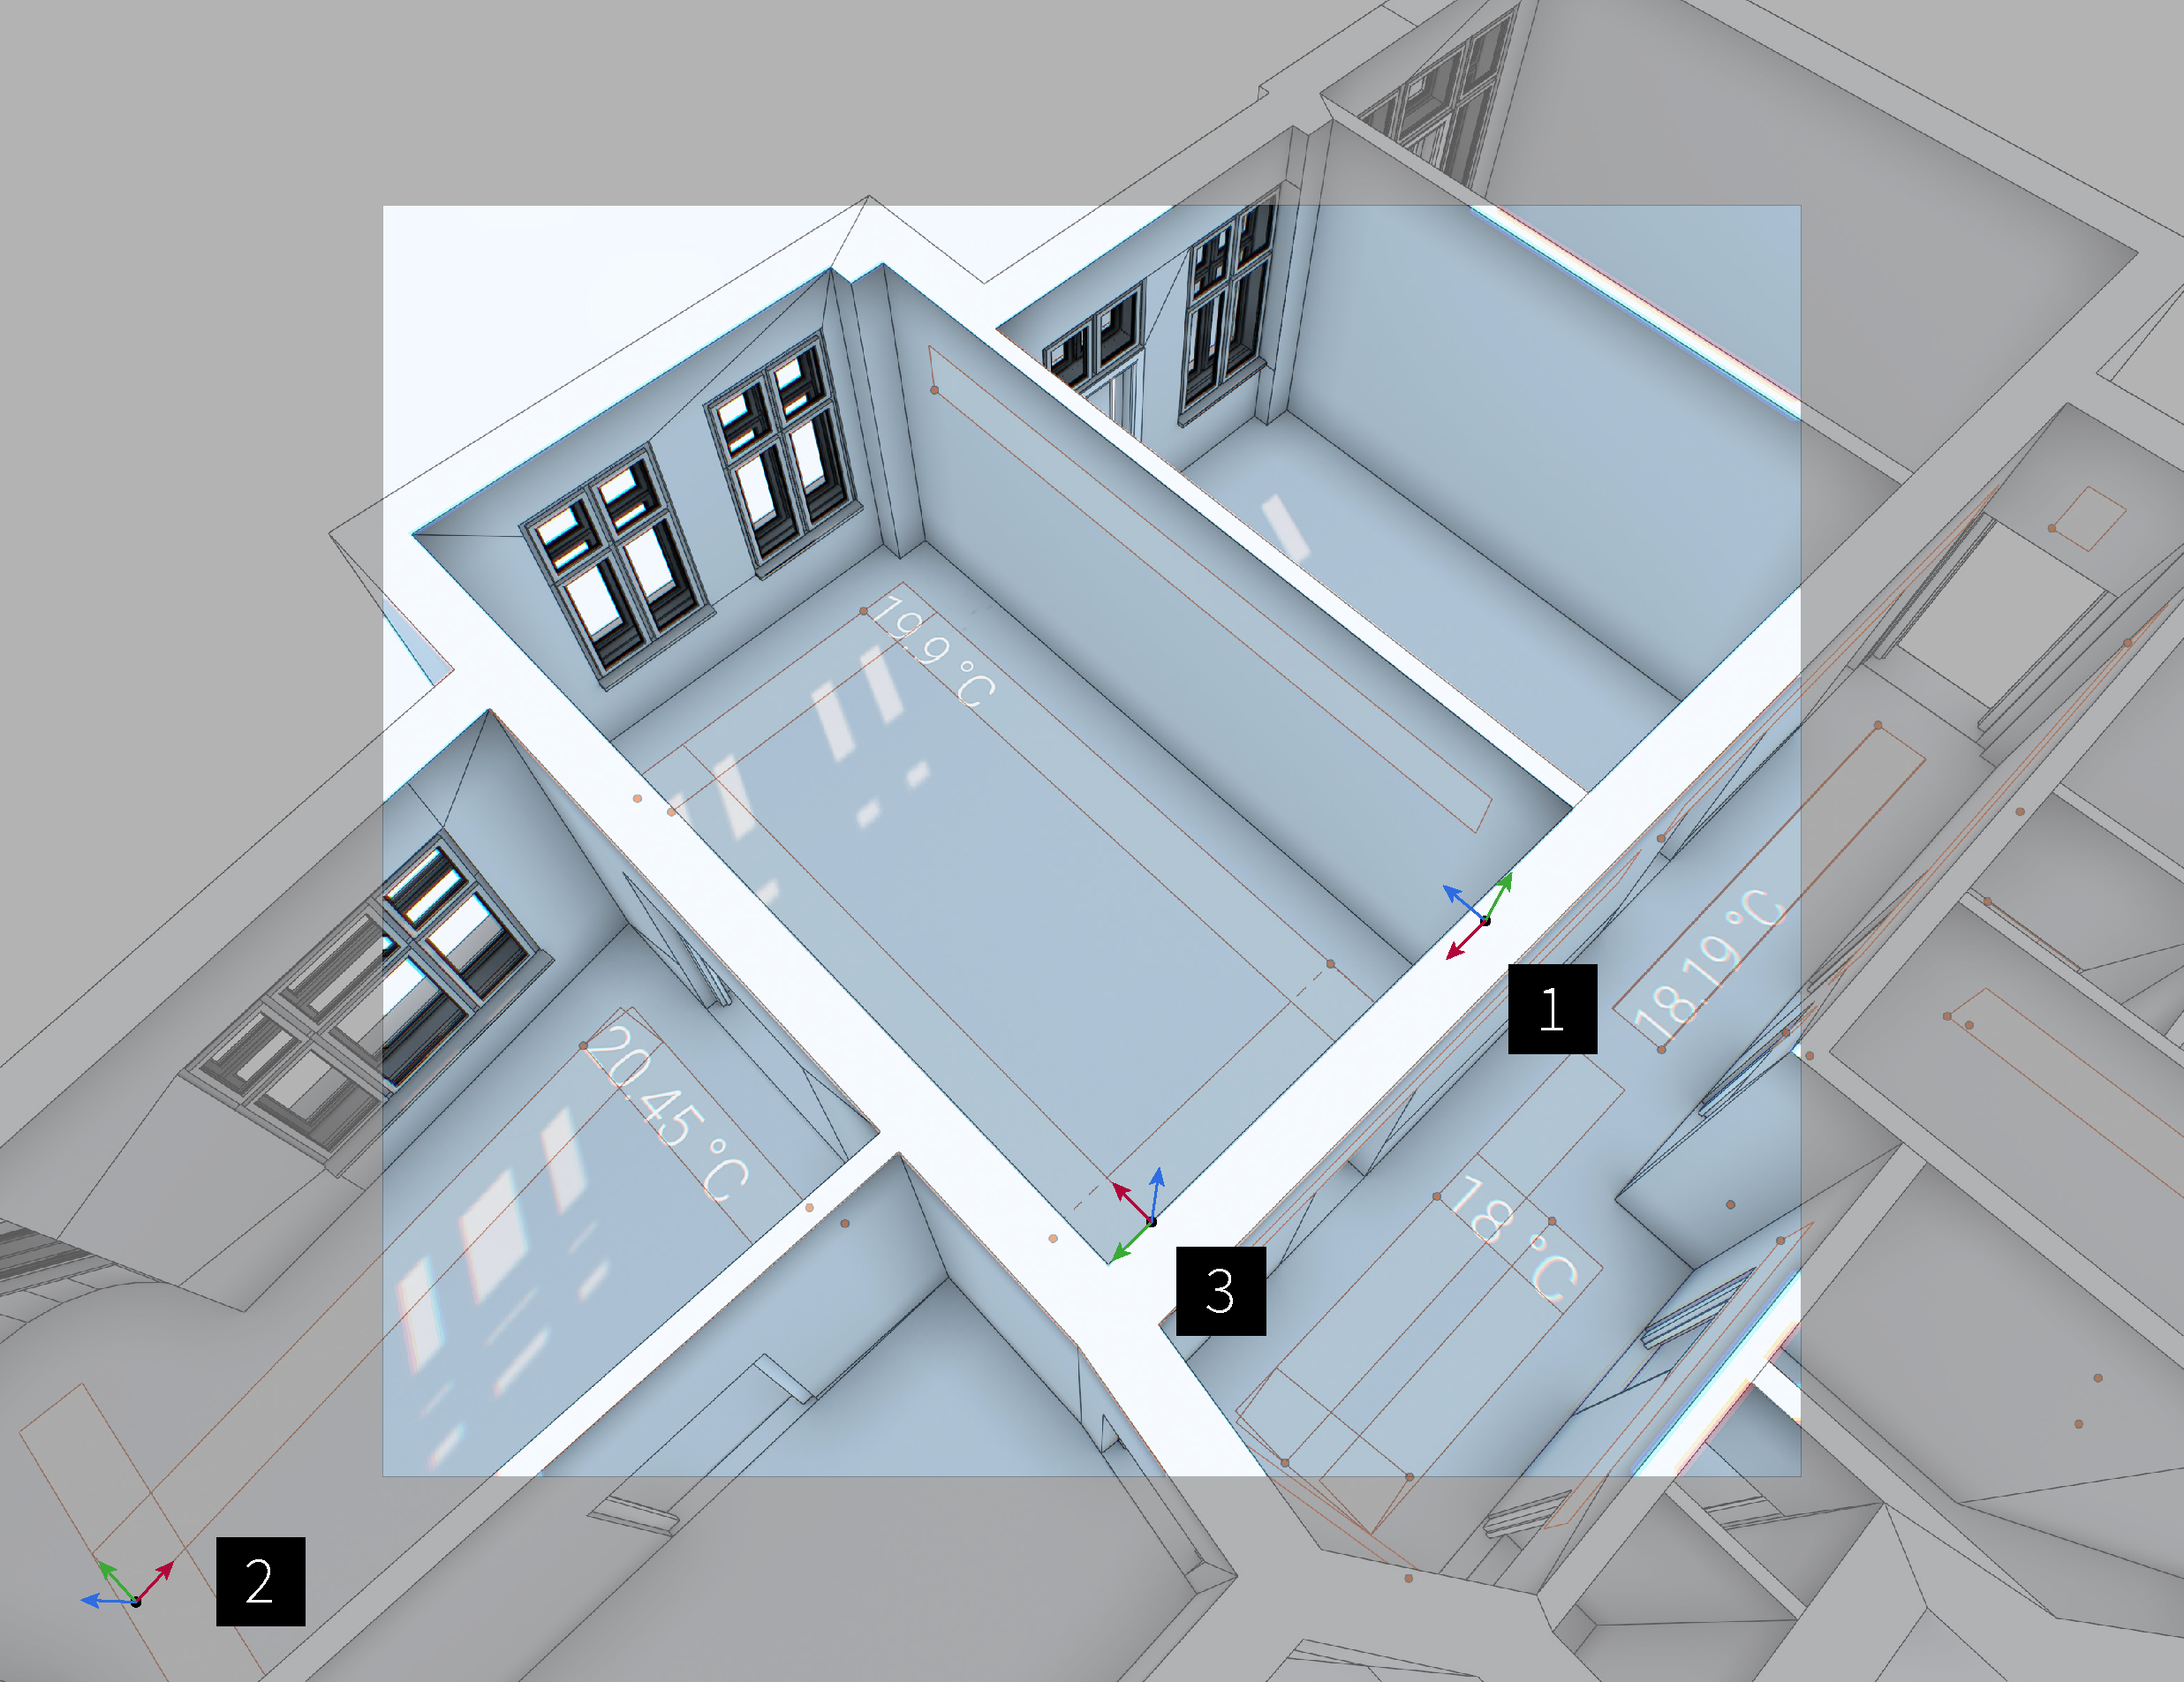
\includegraphics[width=1.0\textwidth]{figures/labelling-scene__step-3.pdf}};%
                        \spy [white] on ($(step3.center)+(+0.28, -1.475)$) in node [fill=white] at ($(-2.1, +1.2)+(step3.center)$);
                    \end{tikzpicture}
                }
                \only<4>{
                    \begin{tikzpicture}[spy using outlines={white, rectangle, magnification=3.0, size=88, line width=2.0pt, connect spies, every spy on node/.append style={line width=1.0pt}},inner sep=0pt, outer sep=0pt]
                        \node[anchor=west](step4) at (0,0) {%
                            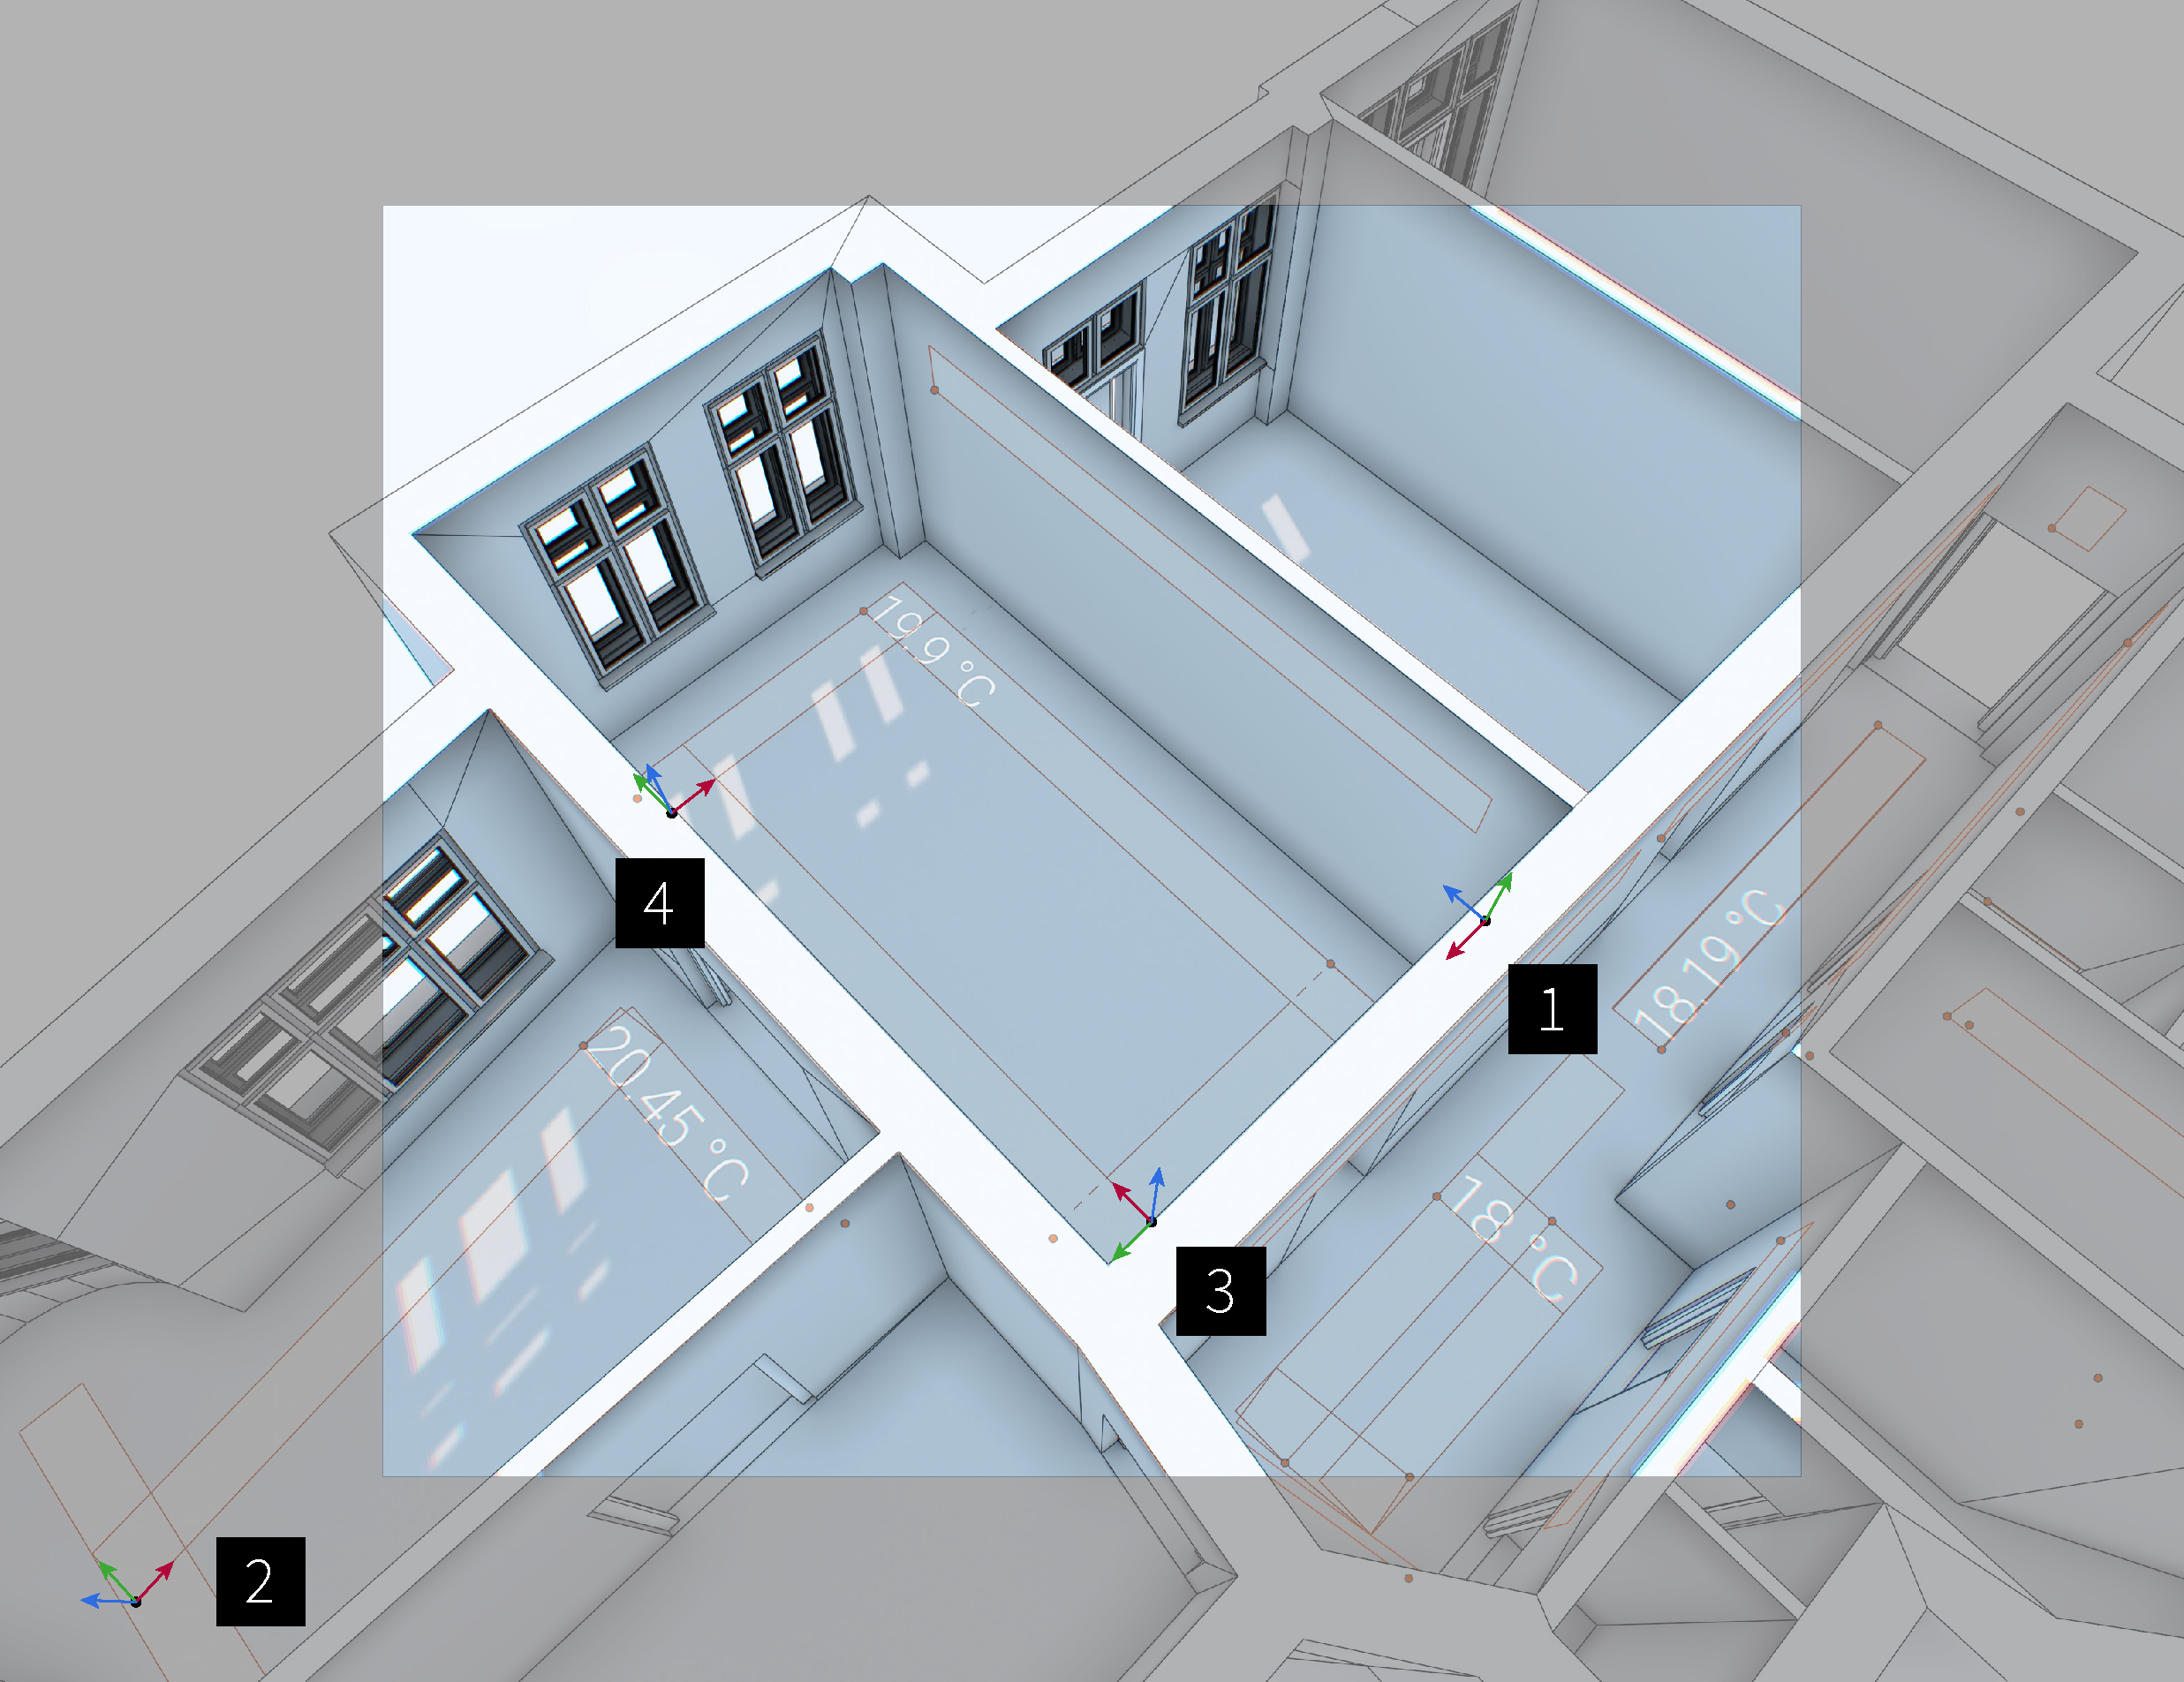
\includegraphics[width=1.0\textwidth]{figures/labelling-scene__step-4.pdf}};%
                        \spy [white] on ($(step4.center)+(-1.415, -0.02)$) in node [fill=white] at ($(+2.1, +1.2)+(step4.center)$);
                    \end{tikzpicture}
                }
                \only<5>{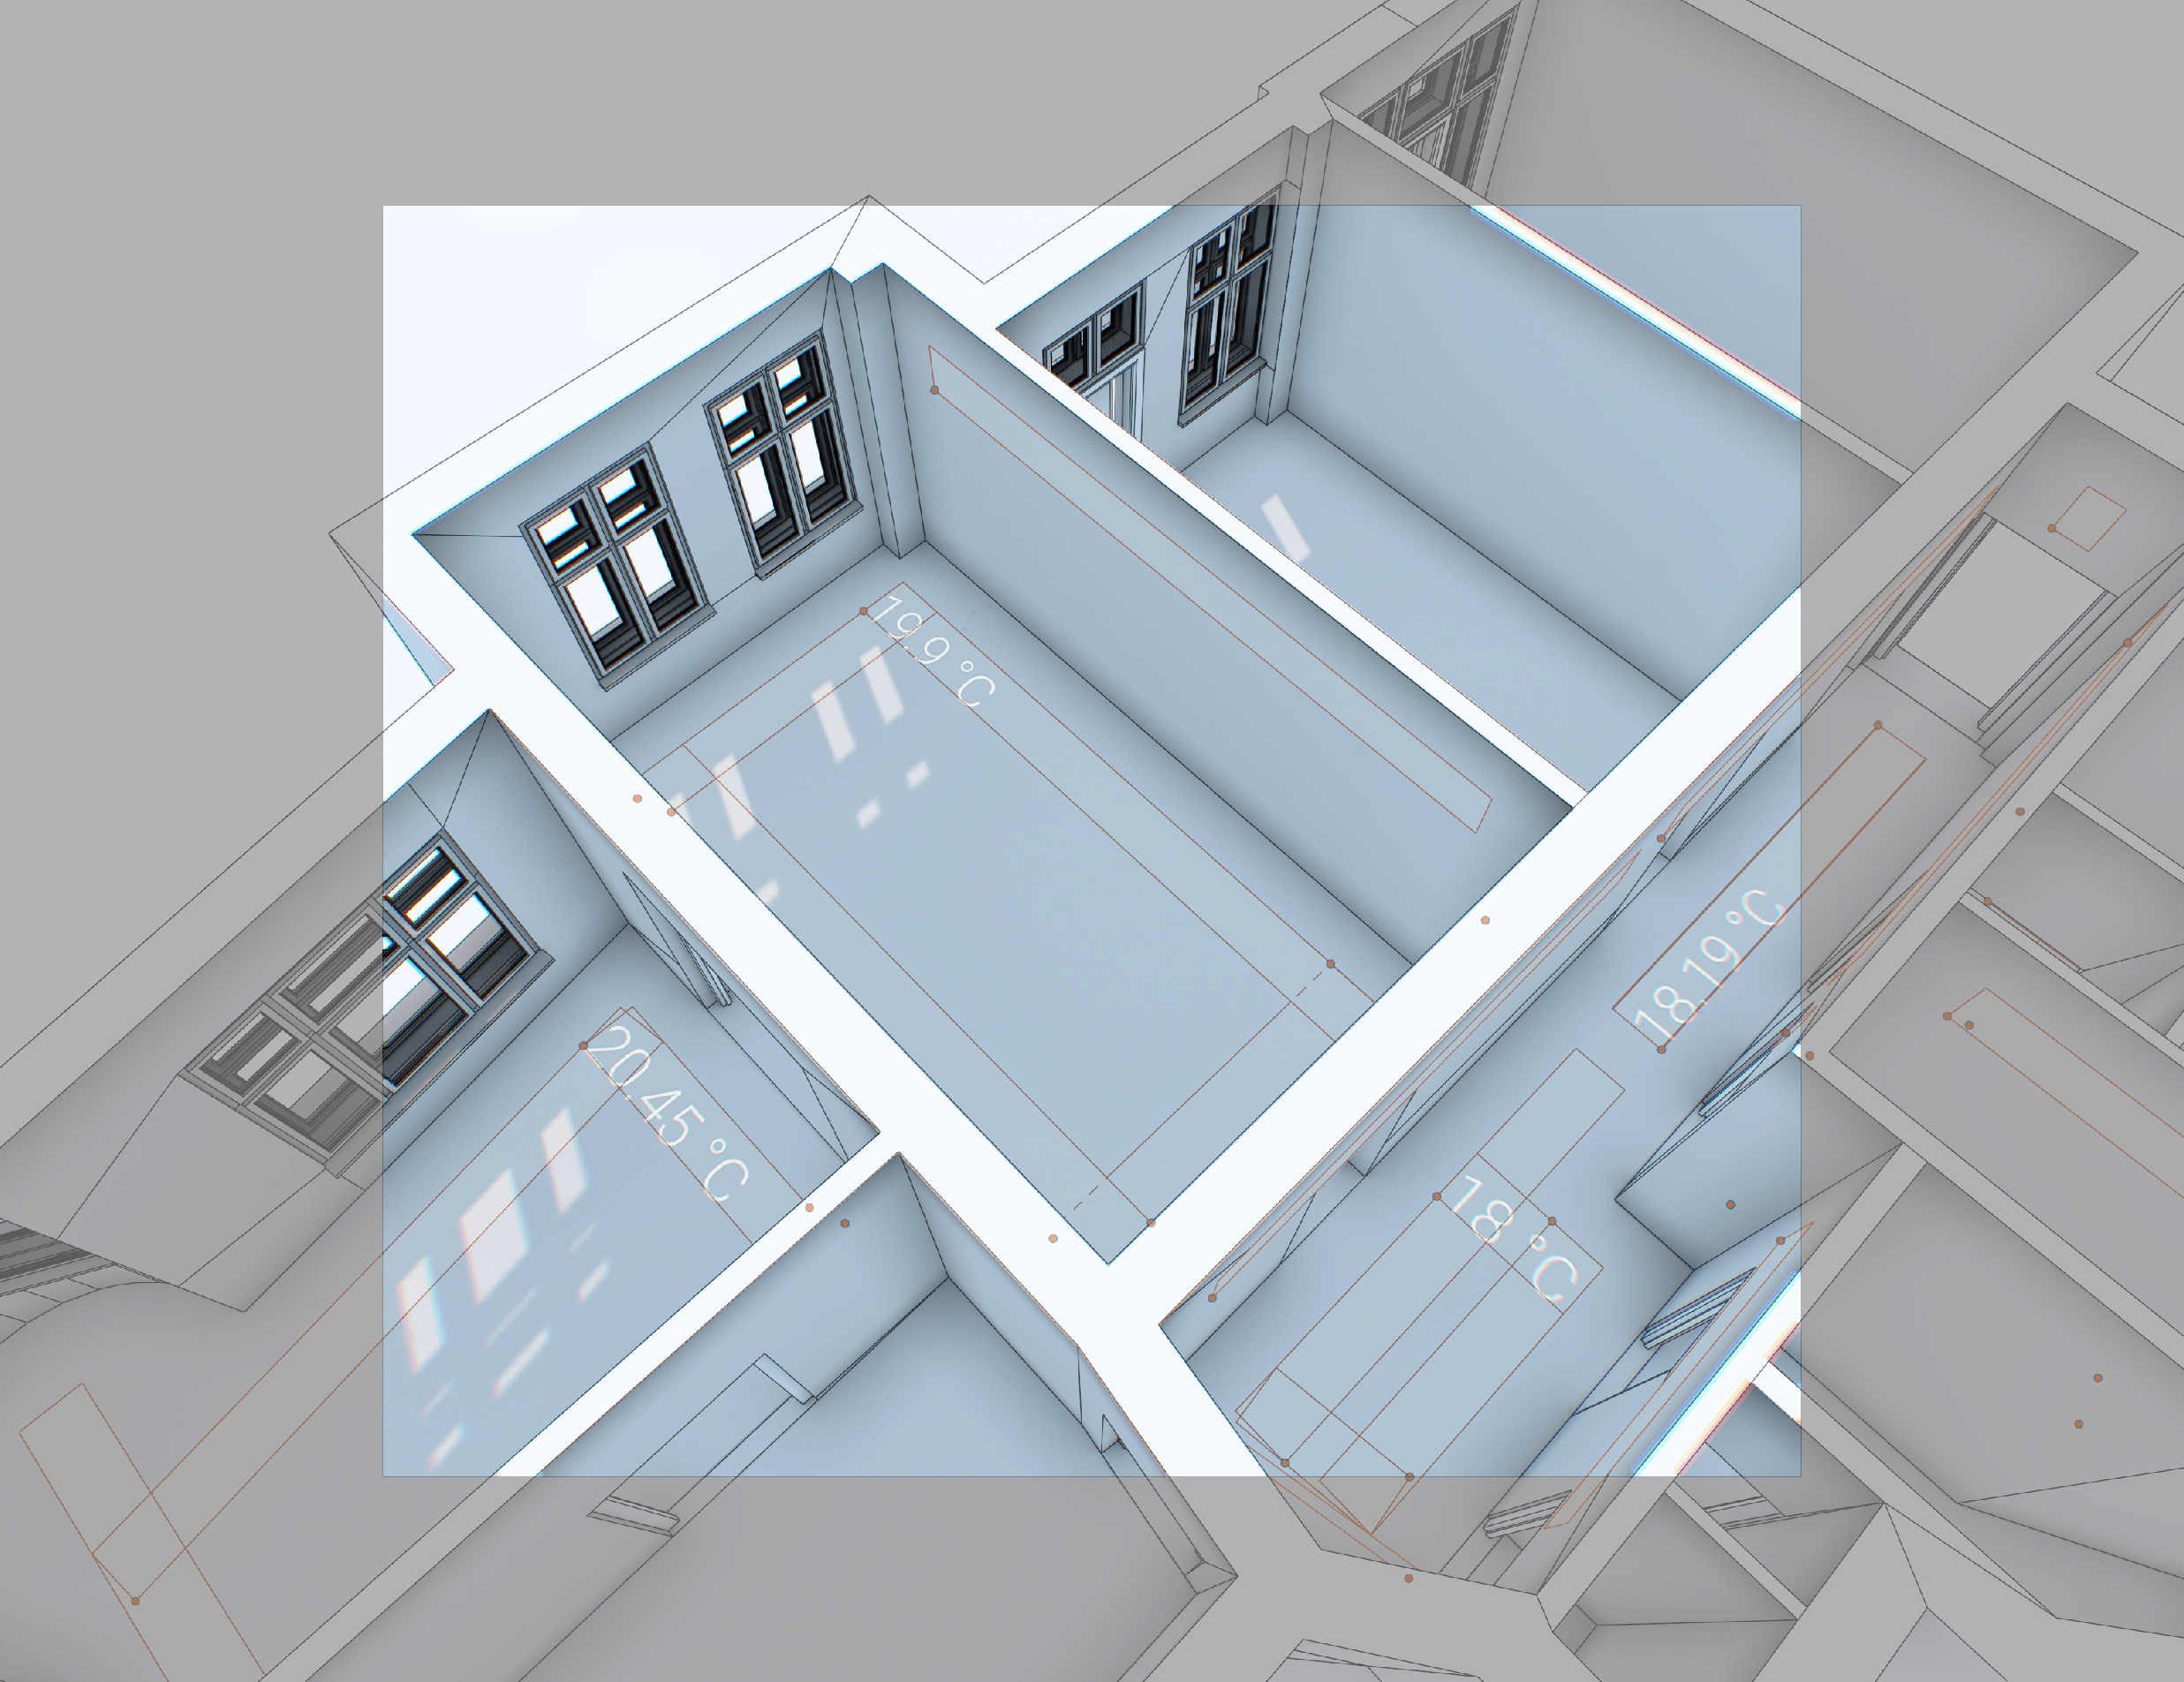
\includegraphics[width=1.0\textwidth]{figures/labelling-scene__result_blank.pdf}}
            \end{figure}
            
        \end{column}
    \end{columns}

\end{frame}

\begin{frame}[t]{\textbf{Future Work}}

    \begin{columns}[T]
        \begin{column}{0.618\textwidth}
            Potential areas for follow-up work include:
                \begin{itemize}
                    \item Extension to larger buildings and industry facilities
                    \item Optimization of sensor amount and distances~\cite{jedermann2009-minimum} 
                    \item Simplification of the manual 3D~floor plan creation
                \end{itemize}
            \smallskip
            \begin{figure}
                \centering
                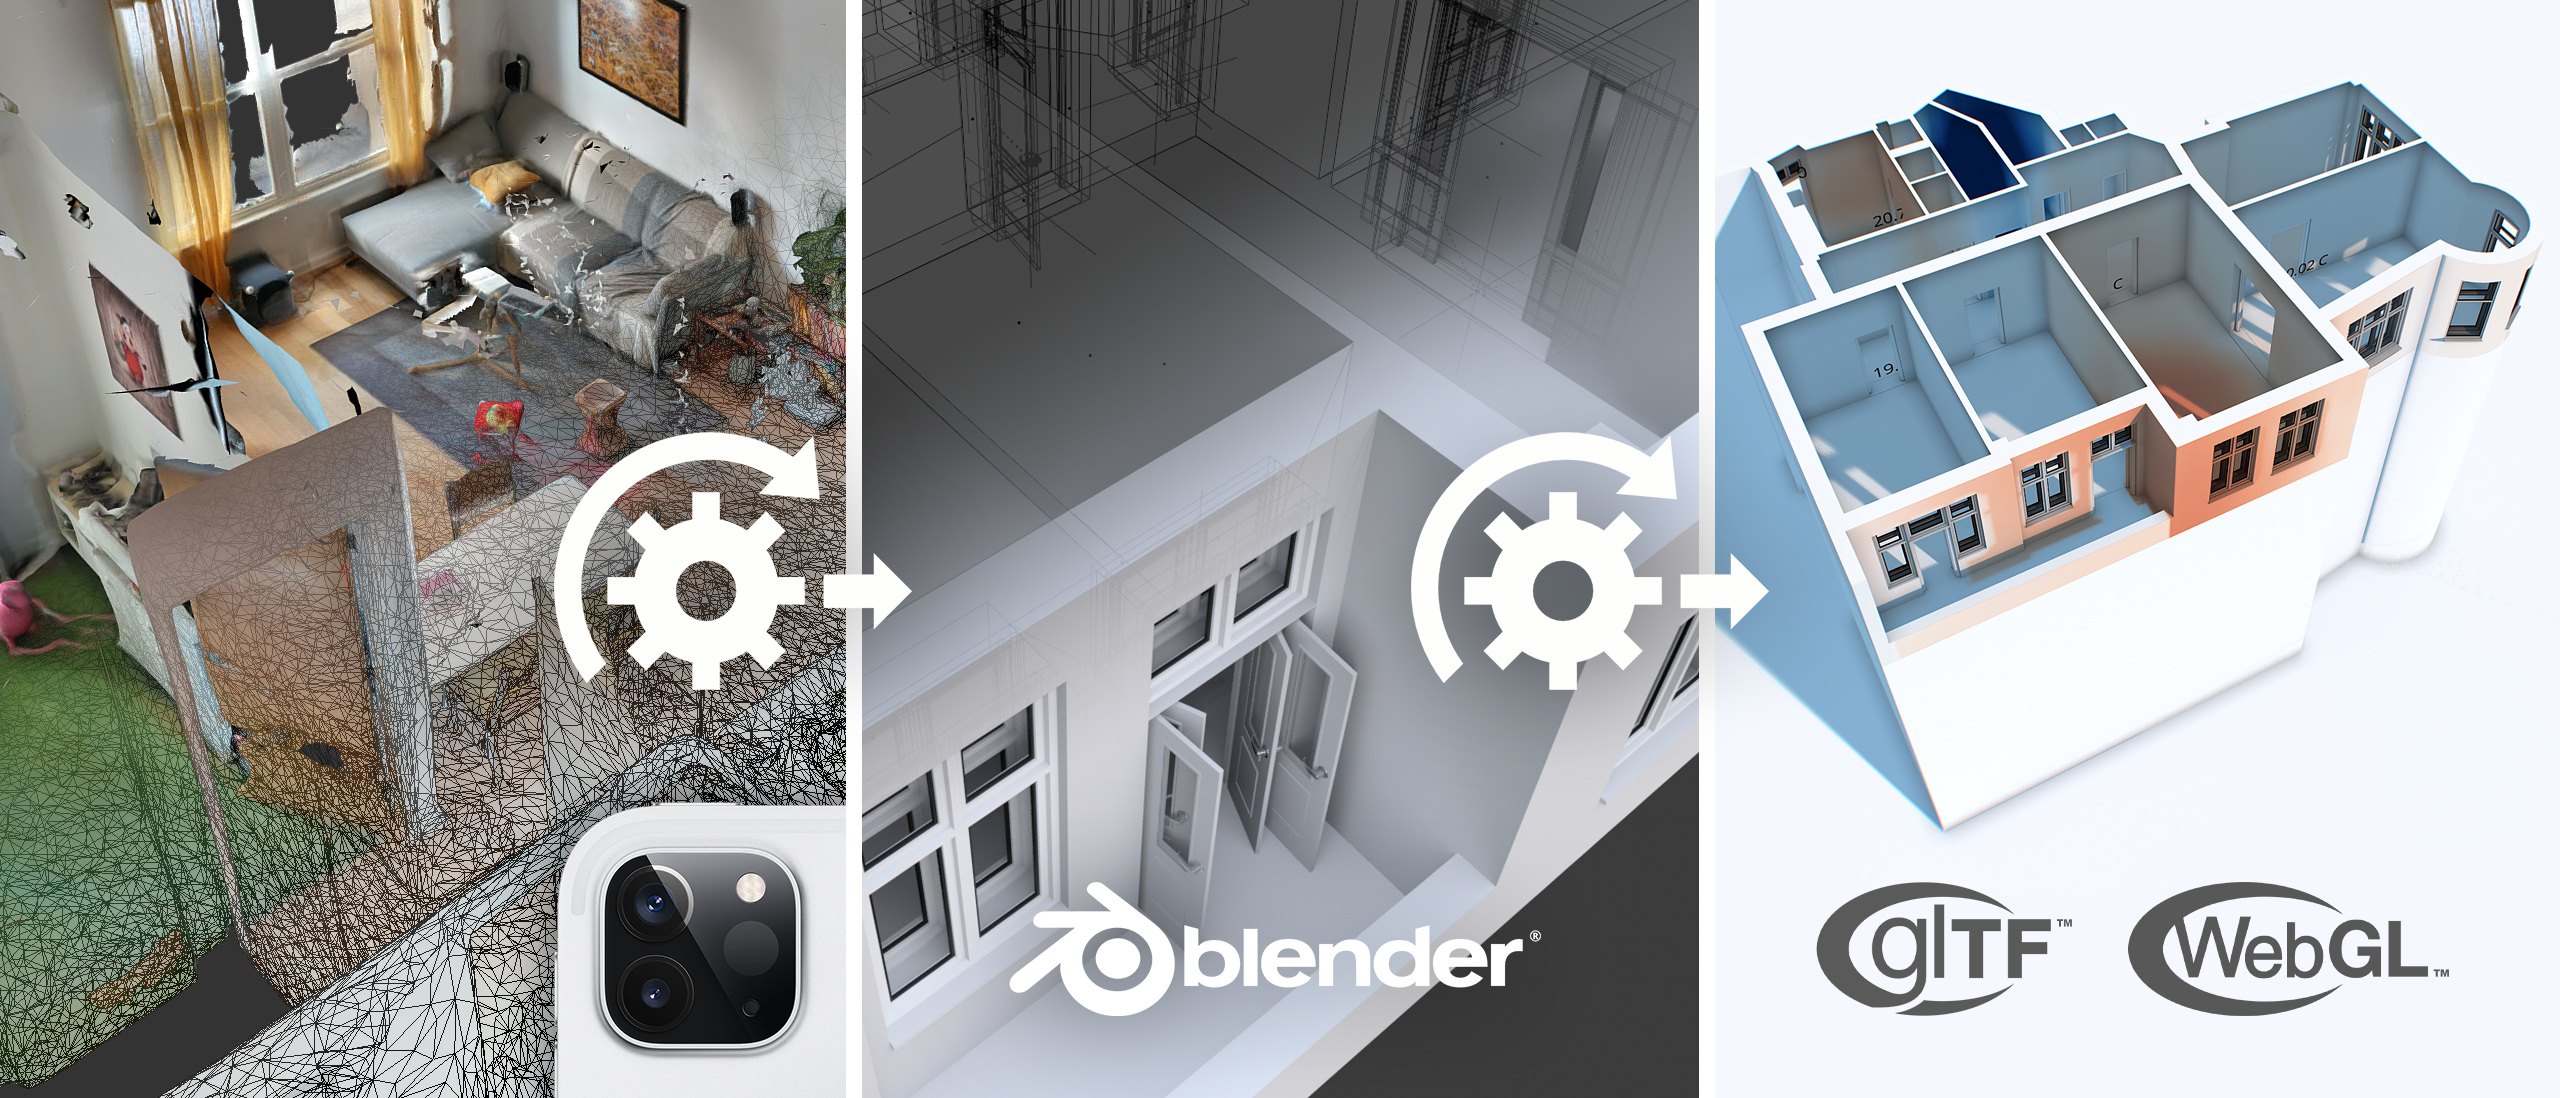
\includegraphics[width=1.0\textwidth]{figures/future-work-1.png}
                \caption*{LiDAR-based capture and preprocessing of 3D floor plans}
            \end{figure}
        \end{column}
        \begin{column}{0.332\textwidth}
            \begin{figure}
                \centering
                \begin{tikzpicture}
                    \node[inner sep=0pt] (berlin-city-model) at (0,0)
                    {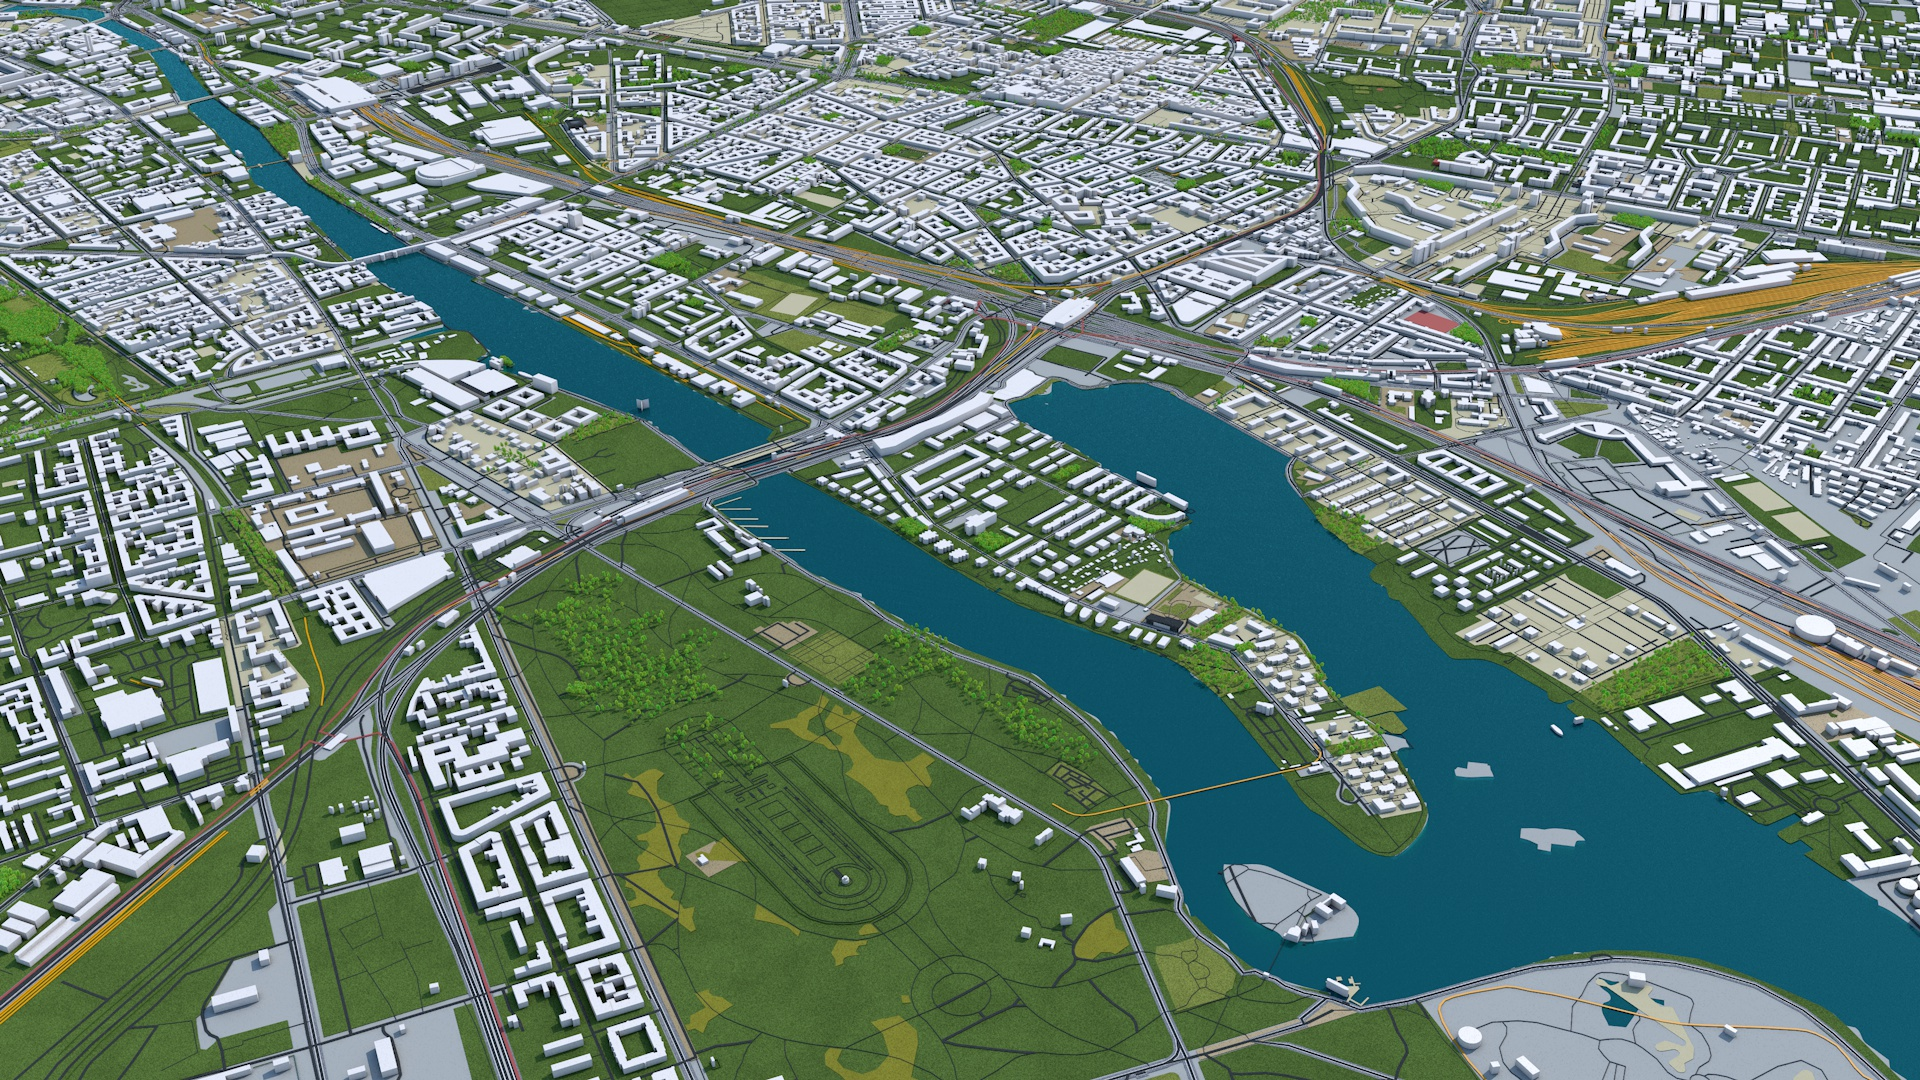
\includegraphics[trim=495 0 495  0, clip,width=\textwidth]{figures/flippednormals_berlin_10-24.jpg}};
                    \node[
                        minimum height=0.55cm,
                        minimum width=0.55cm,
                        anchor=south west,
                        fill=white,
                        shape=rectangle with rounded corners,
                        rectangle with rounded corners north west=0pt,
                        rectangle with rounded corners south west=0pt,
                        rectangle with rounded corners north east=2mm,
                        rectangle with rounded corners south east=0pt,
                        text width=0.53cm,
                    ] at (berlin-city-model.south west) (bg) {};
                    \node[anchor=south west,inner sep=1pt] at (bg.south west) 
                    {\cite{berlin-city-model-screenshot}};
                \end{tikzpicture}\\
                \caption*{Simplified 3D city model for visual embedding of the building}
            \end{figure}
        \end{column}
    \end{columns}

\end{frame}

{
\usebackgroundtemplate{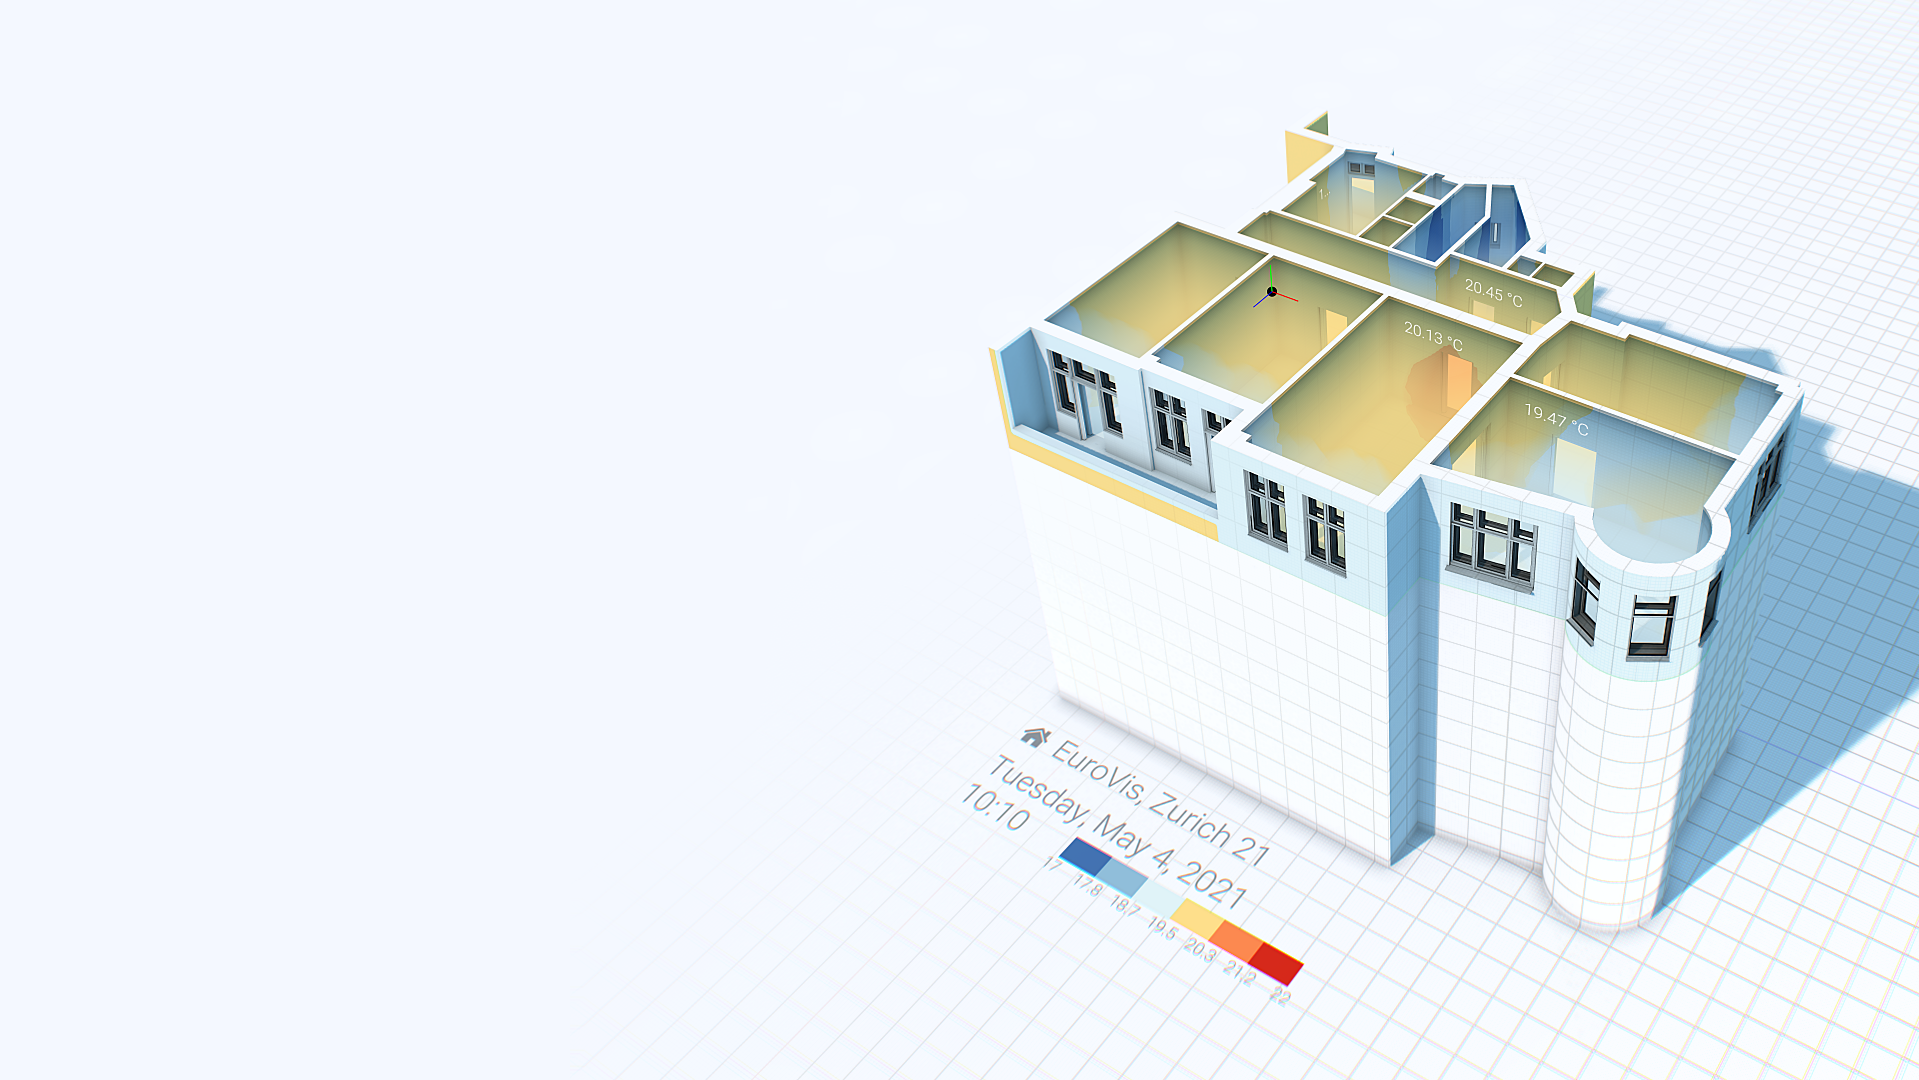
\includegraphics[width=\paperwidth]{figures/contact-bg.png}}

\begin{frame}[t]{\textbf{Questions \& Comments are Welcome!}}

    \begin{columns}[T]
        
        \begin{column}{0.4\textwidth}

        The \textbf{prototype} is available at
        \textbf{\href{https://roomcanvas.dev}{https://roomcanvas.dev}}
        \medskip
        
        The \textbf{toolkit} is/will be available at
        \href{https://source.roomcanvas.dev}{https://source.roomcanvas.dev}
        \bigskip

        For further questions, comments, and collaborations feel free to contact us: 
        \smallskip
        
        \textbf{Bastian König}\\
        \href{mailto:bastian.koenig@student.hpi.de}{bastian.koenig@student.hpi.de}\\
        \smallskip
        
        \textbf{Daniel Limberger}\\
        \href{mailto:daniel.limberger@hpi.de}{daniel.limberger@hpi.de}\\
        \href{tel:+4933155093907}{+49~331~5509-3907}
        \bigskip

        \scriptsize
        Hasso Plattner Institute, University of Potsdam\\
        Prof.-Dr.-Helmert-Str. 2-3 \\
        14482 Potsdam, Germany

        \end{column}
        
        \begin{column}{0.54\textwidth}
        
        \end{column}

    \end{columns}

\end{frame}
}

\begin{frame}[allowframebreaks]
        \frametitle{\textbf{References}\enspace{}|\hspace{.2em}}
        \bibliographystyle{eg-alpha-doi}
        \bibliography{references-eurovis.bib}
\end{frame}

{
\usebackgroundtemplate{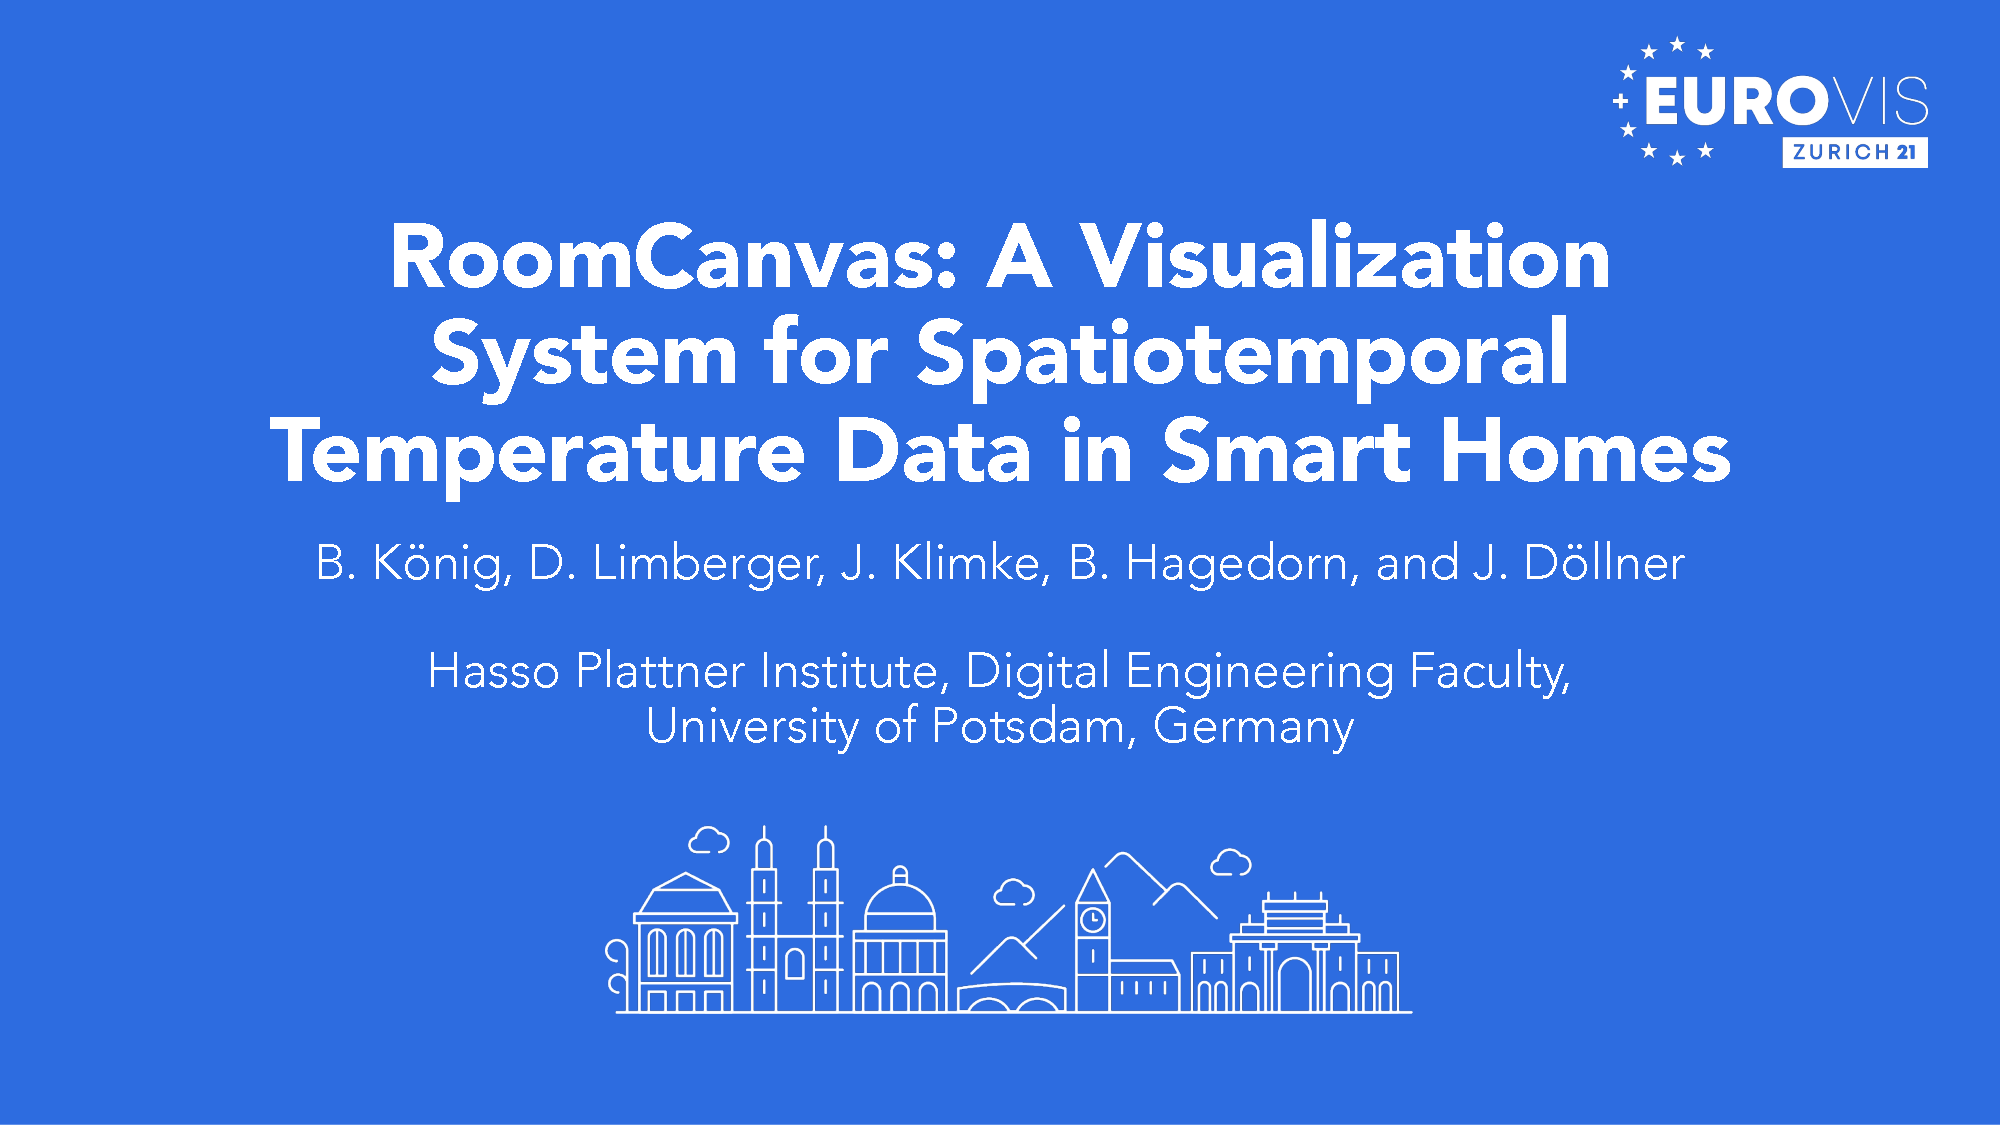
\includegraphics[width=\paperwidth]{figures/EuroVis21.pdf}}
\begin{frame}[plain]
\end{frame} 
}

\end{document}

